% ****** Start of file aipsamp.tex ****m*
%
%   This file is part of the AIP files in the AIP distribution for REVTeX 4.
%   Version 4.1 of REVTeX, October 2009
%
%   Copyright (c) 2009 American Institute of Physics.
%
%   See the AIP README file for restrictions and more information.
%
% TeX'ing this file requires that you have AMS-LaTeX 2.0 installed
% as well as the rest of the prerequisites for REVTeX 4.1
% 
% It also requires running BibTeX. The commands are as follows:
%
%  1)  latex  aipsamp
%  2)  bibtex aipsamp
%  3)  latex  aipsamp
%  4)  latex  aipsamp
%
% Use this file as a source of example code for your aip document.
% Use the file aiptemplate.tex as a template for your document.
\documentclass[%
 pra,
% jmp,
% bmf,
% sd,
% rsi,
 amsmath,amssymb,
%preprint,%
 reprint,%
%author-year,%
%author-numerical,%
% Conference Proceedings
]{revtex4-1}

\usepackage{graphicx}% Include figure files
%\usepackage{dcolumn}% Align table columns on decimal point
\usepackage{bm}% bold math
\usepackage{fixme}
%\usepackage[mathlines]{lineno}% Enable numbering of text and display math
%\linenumbers\relax % Commence numbering lines
\usepackage{hyperref}
\usepackage{kbordermatrix}% http://www.hss.caltech.edu/~kcb/TeX/kbordermatrix.sty
\usepackage[utf8]{inputenc}
\usepackage[T1]{fontenc}
\usepackage{mathptmx}
\usepackage{lipsum}
\usepackage{amsmath}
\usepackage{physics}
\usepackage{xparse}
\usepackage{bbm}
\usepackage{xcolor}


%\usepackage{multirow}
%\usepackage{makecell}
\graphicspath{{Pictures/}}

\renewcommand*{\figureautorefname}{Fig.}
\renewcommand*{\equationautorefname}{Eq.}

\newcommand{\mytitile}{Light-dressing of a 
diatomic supercondufcing artificial molecule}

\begin{document}
	\preprint{AIP/123-QED}
	
	\title[\mytitile]{\mytitile\\~}
	\author{G.P. Fedorov}
	\email{gleb.fedorov@phystech.edu}
	
	\affiliation{ 
		Russian Quantum Center, Skolkovo village, Russia
	}%
	\affiliation{ 
		Moscow Institute of Physics and Technology, Dolgoprundiy, Russia
	}
	\affiliation{
		National University of Science and Technology MISIS, Moscow, Russia
	}%
	\author{V.B. Yursa}
	\affiliation{ 
		Skolkovo Institute of Science and 
		Technology, Moscow, Russian Federation
	}%

\affiliation{ 
	Moscow Institute of Physics and Technology, 
	Dolgoprundiy, Russia
}%
	
	\author{A. Efimov}
	
	\affiliation{ 
		Moscow Institute of Physics and Technology, Dolgoprundiy, Russia
	}%
	
	\author{K. Shiianov}

	\affiliation{ 
		Moscow Institute of Physics and Technology, Dolgoprundiy, Russia
	}%

	\author{A. Yu. Dmitriev}
	\affiliation{ 
	Moscow Institute of Physics and Technology, Dolgoprundiy, Russia
	}%

	\author{I.A. Rodionov}
	\affiliation{FMN Laboratory, Bauman Moscow 
	State Technical University, Moscow, Russia}
	\affiliation{Dukhov Automatics Research 
	Institute, (VNIIA), Moscow, Russia}
	
	
	\author{A.A. Dobronosova}
	\affiliation{FMN Laboratory, Bauman Moscow 
	State Technical University, Moscow, Russia}
	\affiliation{Dukhov Automatics Research 
	Institute, (VNIIA), Moscow, Russia}
	
	
	\author{D.O. Moskalev}
	\affiliation{FMN Laboratory, Bauman Moscow 
	State Technical University, Moscow, Russia}
	
	
	\author{A.A. Pischimova}
	\affiliation{FMN Laboratory, Bauman Moscow 
	State Technical University, Moscow, Russia}
	\affiliation{Dukhov Automatics Research 
	Institute, (VNIIA), Moscow, Russia}

	\author{O.V. Astafiev}
	\affiliation{ 
		Moscow Institute of Physics and Technology, Dolgoprundiy, Russia 
	}
	\affiliation{Skolkovo Institute of Science 
	and Technology, Moscow, Russian Federation}
	\affiliation{Physics Department, Royal 
	Holloway, University of London, Egham, Surrey 
	TW20 0EX, United Kingdom}
%
	
	
	\date{\today}% It is always \today, today,
	%  but any date may be explicitly specified
	
	
	\begin{abstract}
	In this work, we irradiate a superconducting 
	artificial molecule composed of two 
	magnetic-flux-tunable transmons with 
	microwave light while monitoring its state 
	via joint dispersive readout. At certain 
	fluxes, the molecule demonstrates a complex 
	spectrum deviating qualitatively from the 
	solution of the Schrödinger equation without 
	driving. We reproduce the observed extra 
	spectral lines accurately by numerical 
	simulations, and find them to be a 
	consequence of an Autler-Townes-like effect 
	when a single tone is simultaneously dressing 
	the system and probing the transitions 
	between new eigenstates. We present 
	self-consistent analytical models accounting 
	both these processes at the same time that 
	agree well with both experiment and numerical 
	simulation. This study is an important step 
	towards understanding the behaviour of complex
	systems of many atoms interacting	with strong radiation.
	\end{abstract}
	
	\maketitle
\section{Introduction}





Over the past twenty years, superconducting 
artificial atoms (SAAs) were used in numerous 
experiments in a compelling demonstration of the 
validity of fundamental quantum mechanical 
laws. Due to synthetic nature 
of SAAs, their Hamiltonians can be pre-designed 
and engineered which makes them a particularly 
versatile tool for studies in microwave quantum 
optics \cite{you2011atomic,Qopt_1300refs}. Notably, high controllability
of their parameters allows direct observation of novel physical 
effects previously inaccessible for natural 
systems. 

One of the most prominent milestones that 
superconducting quantum circuits have reached so 
far is the strong coupling with light in {circuit 
QED}\cite{wallraff2004strong, 
chiorescu2004coherent} when the relaxation and decoherence rates 
appear smaller than the Rabi frequency. 
Currently, they are surpassing all other 
implementations of strong coupling in terms of 
coherence\cite{forn2019ultrastrong}. 
However, in sharp contrast with natural atoms and 
molecules, SAAs do not even require confined 
radiation to implement strong coupling with 
light: they may be coupled unprecedently strongly 
to free-propagating electromagnetic waves in 1D 
on-chip waveguides\cite{astafiev2010resonance} 
without using cavities at all. The Rabi frequency 
in this case may reach 50\% of the transition 
frequency\cite{deng2015observation} which is even 
beyond strong coupling 
regime\cite{forn2019ultrastrong}. To correctly 
describe the behaviour of an atom in these 
conditions, the so-called \textit{dressed atom 
approach}\cite{cohen1998atom} is employed when 
the radiation has to be directly included in the 
Hamiltonian and affects its level structure.

So far, experiments with intense driving fields resulting in the dressing effects in on-chip quantum optics  were 
focused on single artificial 
atoms\cite{baur2009measurement, 
sillanpaa2009autler, astafiev2010resonance, 
novikov2013autler, suri2013observation, 
koshino2013observation, 
braumuller2015multiphoton, peng2018vacuum, 
gasparinetti2019two}. In all these works, light 
dressing of the atom manifests itself through 
Mollow triplets or Autler-Townes (A-T) splittings of 
different kinds. However, despite the recent 
successes in control of large arrays of 
interacting SAAs\cite{Song574, ye2019propagation, 
arute2019quantum}, there were, up to our best 
knowledge, no experiments concerning interaction 
of similar composite structures with intense driving field. While there were studies on dressing 
of multi-atomic systems in a 
cavity\cite{fink2009dressed, 
macha2014implementation, shulga2017observation, 
yang2018probing}, their interaction with external dressing field is not less attractive since its 
frequency may be easily tuned to observe various 
absorption processes for arbitrary configurations 
of the system parameters.

In this work, we study a pair of strongly coupled 
artificial atoms: a superconducting artificial 
molecule\cite{kou2017fluxonium} (SAM). We use two 
Xmon-type\cite{barends2013coherent} 
transmons\cite{koch2007charge} interacting with 
each other through a cavity 
bus\cite{majer2007coupling}. Microwave radiation 
is applied to this system through an on-chip 
coplanar antenna while its state can be 
monitored by joint dispersive readout using the 
same coupling cavity\cite{chow2010detecting}. We 
find that strong interaction with microwaves not 
only results in multiphoton transitions of 
various orders between SAM states, but also 
significantly modifies its level structure. Even 
in a simple diatomic molecule, this leads to 
complex Autler-Townes-like effects involving 
single- and multiphoton  transitions that can 
only be explained in the dressed picture. We note 
that although the A-T splittings have been 
investigated before in a wide range of quantum 
systems (including natural 
molecules\cite{tamarat1995pump, 
ahmed2012autler}), we find qualitatively new 
spectral manifestations of light dressing when 
SAAs are irradiated unequally. We note that there 
were no such experiments with natural molecules, 
which could in principle demonstrate same 
effects, because they lack controllability and 
coherence of superconducting quantum devices, and 
previous studies of SAAs under strong driving field 
either involved just a single atom or have 
demonstrated only the standard spectral 
signatures known from the quantum optics (see 
Appendix \ref{sec:3-level-at}). 

Besides its fundamental importance, this 
experiment may be useful for future quantum 
computers: a quantum engineer should account for 
the observed behaviours carefully controlling the 
driving power (for instance, as we will show, the 
bSWAP gate\cite{poletto2012entanglement} is 
directly affected by light dressing).

The manuscript consists of four main parts and an 
Appendix. Section I is this introduction; Section 
II is devoted to the approaches that were used in 
our study; Section III contains the results of 
our experimental and theoretical research, 
including numerical simulations and analytical 
analysis; finally, in Section IV we make a 
conclusion of our work and discuss future 
prospects. The Appendix contains important 
details of the theoretical framework that we use.

\section{Methods}

\subsection{Device design and control}
We have designed the SAM as a pair of transmon 
(Xmon) SAAs with asymmetric 
SQUIDs\cite{hutchings2017tunable} ($E^1_{J, 
\sum}/h = 24.3$ GHz, $E^2_{J,\sum}/h = 18.3$ GHz, 
$E^{1,2}_C/h = 220$ MHz, $d^{1,2} =0.75$) coupled 
to a single notch-type\cite{probst2015efficient} 
$\lambda/4$ resonator ($f_r = 7$ GHz, $\kappa = 
1/100\ \text{ns}^{-1}$) which both 
couples\cite{majer2007coupling} the transmons and 
allows joint readout \cite{chow2010detecting} of 
their states. In \autoref{fig:experiment}~(a), 
the optical photograph of the device is shown, where the layout of the components is presented. The 
resonator in its upper part is connected to a 
coplanar waveguide through which the readout is 
performed. In its lower part, it is coupled to 
the transmons by a dual 
``claw''\cite{barends2013coherent} coupler. Flux 
lines that allow independent control of the 
transmon frequencies are coming from the sides. 
Finally, the excitation waveguide coming from 
below directs microwave signal towards the SAM. 
In \autoref{fig:experiment}~(b), the equivalent 
electrical circuit of the device is shown. The 
resonator fundamental mode is approximated as an 
LC-circuit (in the middle), the transmons are 
shown in color on the sides; their SQUIDs are 
represented as tunable Josephson junctions. A 
capacitively coupled excitation line is also 
shown in green. Finally, in 
\autoref{fig:experiment}~(c) we show 
schematically the frequencies of the transmons 
depending on electric current $I$ which we apply 
to an external coil wound around the sample 
holder. Since the effective junction of the first 
transmon is larger, its spectrum (orange) lies 
higher in frequency than the spectrum of the 
second transmon (blue). Using individual 
flux-control lines, it is possible to align the 
SAAs so that the lower sweet-spot of the orange 
transmon is just below the upper sweet-spot of 
the blue transmon (see the dashed rectangle,  
\autoref{fig:experiment}~(c)). This configuration 
is, as we will show in the following, convenient 
to track the energies of highly excited levels 
via multi-photon transitions in a single 
spectroscopic scan. Additionally, the transmons 
are better protected from the flux noise in this 
area being close to their sweet spots.



\begin{figure}
	 	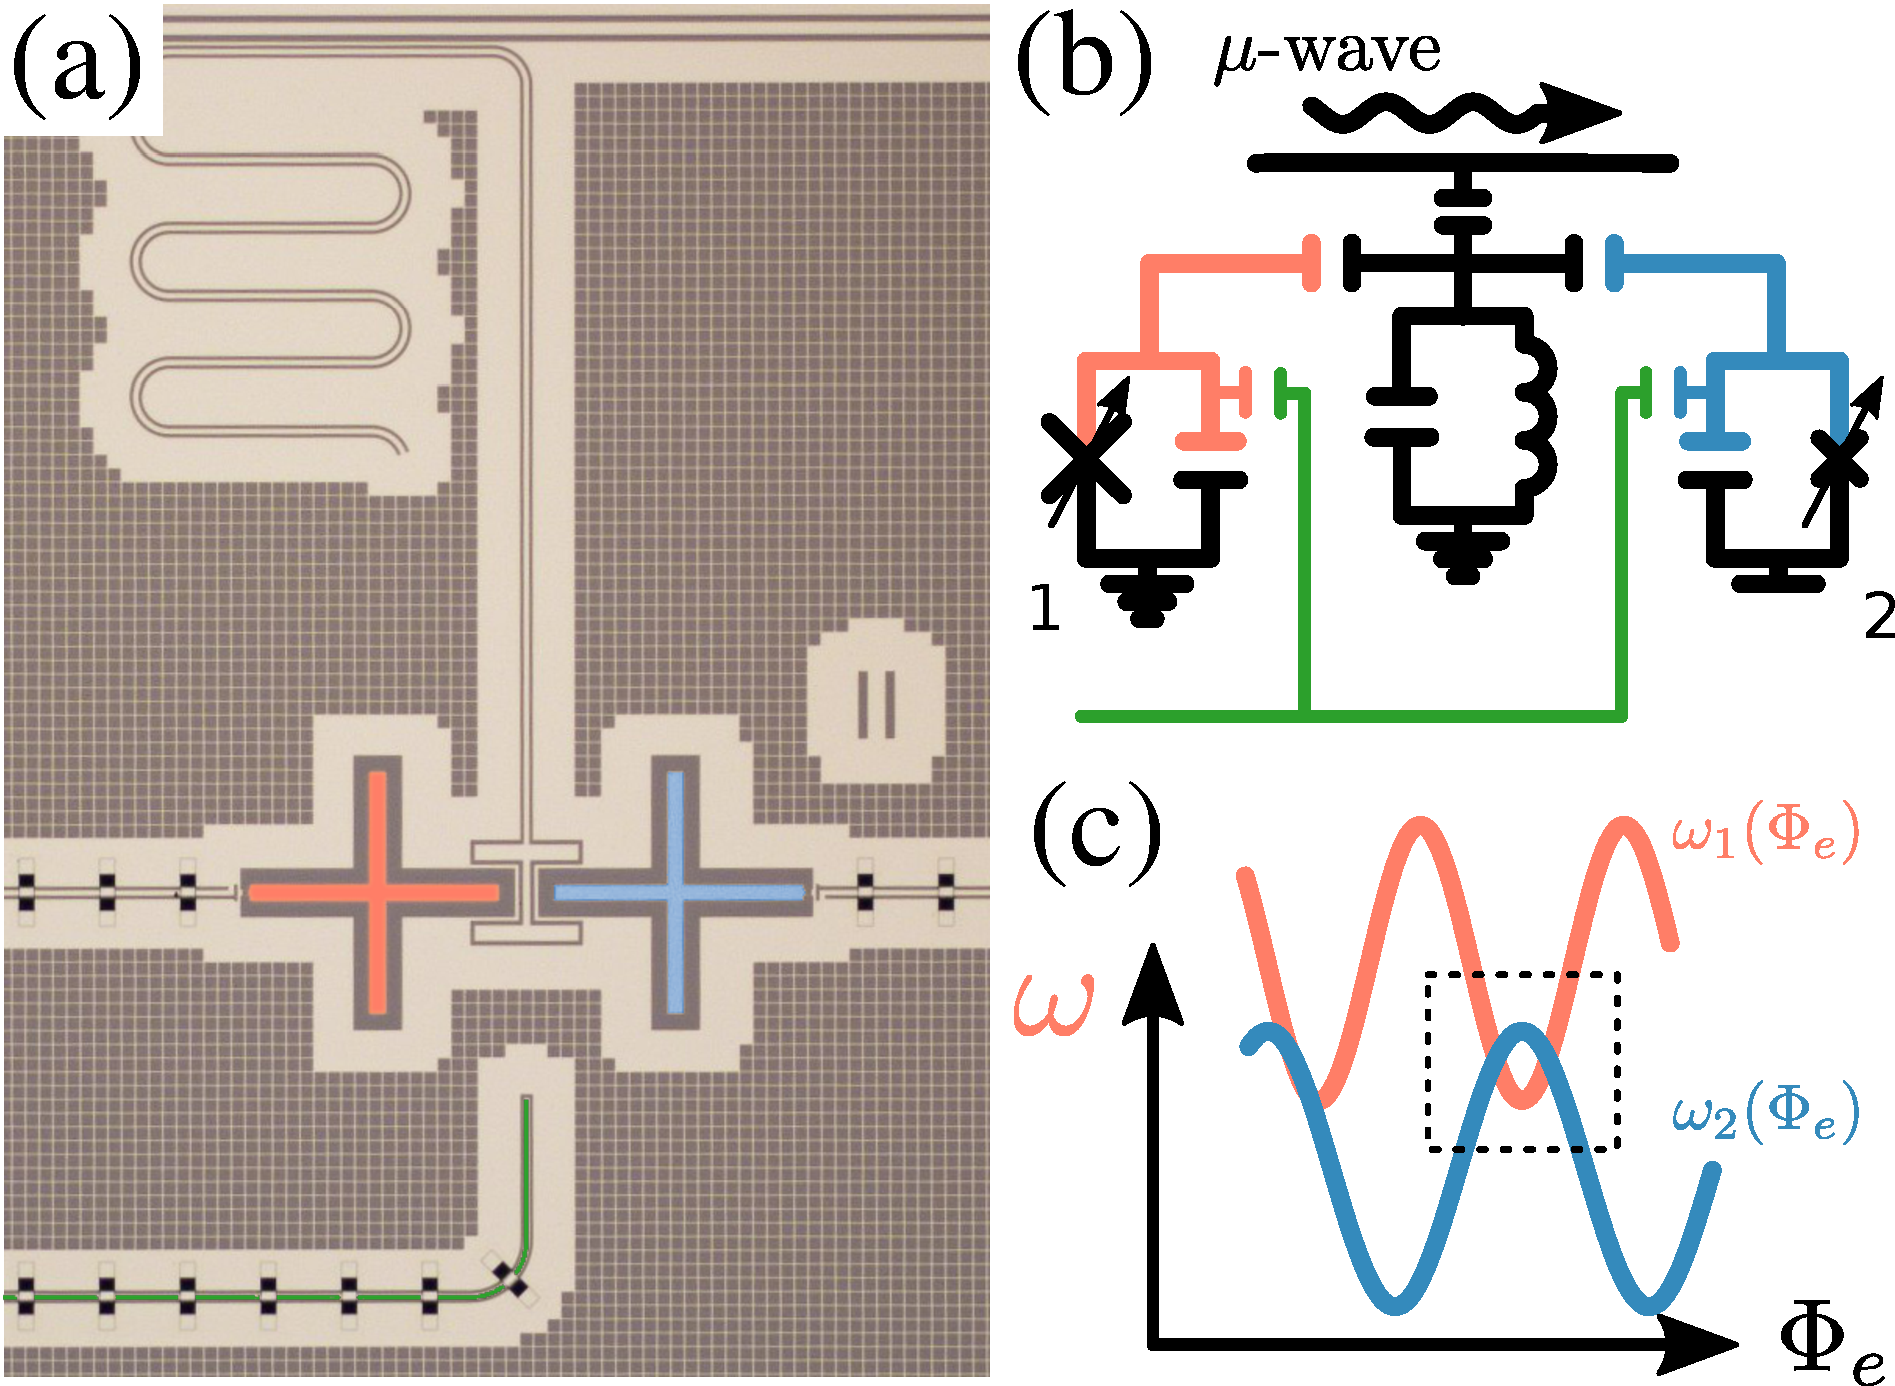
\includegraphics[width=\linewidth]{experiment_2}
	\caption{\textbf{(a)} Optical photograph of 
	the device (false coloured). Two transmons 
	(orange, 1 and blue, 2) are coupled 
	capacitively to a $\lambda/4$ coplanar 
	resonator. Frequency control lines come from 
	both sides, and from below a waveguide for 
	microwave excitation  is connected (green). 
	\textbf{(b)} The equivalent electrical 
	circuit. Tunable Josephson junctions are 
	SQUIDs with magnetic flux control. 
	\textbf{(c)} Frequencies of the fundamental 
	transitions of the transmons $\omega_1(I)$ 
	and $\omega_2(I)$ depending on the current 
	$I$ in an external coil when correctly 
	aligned by the individual flux control lines. 
	In this work, we focus on the area inside the 
	dashed rectangle.}
	\label{fig:experiment}
\end{figure}


\begin{table}
	\begin{ruledtabular}
	\begin{tabular}{rll}
	Parameter & Transmon 1  & Transmon 2\\\hline
	$\omega/2\pi$ [GHz] & 5.12 - 6.3  & 4 - 5.45\\
	$\alpha/2\pi$ [MHz] & -220 & -220 \\
	$T_1$ [$\mu$s]  & 6.82 &  4.41 \\
	$T_2^*$ [$\mu$s]  & 5.14  &  3.33\\\hline
	$J/2\pi$ [MHz] &\multicolumn{2}{c}{8} 
	\end{tabular}
	\end{ruledtabular}
	\caption{SAM parameters. Transmons are only 
	different in the frequency tuning range and 
	coherence times measured in the lower sweet 
	spot for the 1\textsuperscript{st} one and in 
	the higher sweet spot for the 
	2\textsuperscript{nd}. The coupling strength 
	$J$ depends on the transmon frequencies and 
	is specified here for $\omega_1/2\pi = 
	\omega_2/2\pi = 5.32$ GHz.}
	\label{tab:parameters}
\end{table}


\subsection{Theoretical background}

A single transmon SAA can be regarded as an 
oscillator with a quartic perturbation describing 
the leading-order anharmonicity. Therefore, in 
the main text we do not use the charge and phase 
operators and write down its Hamiltonian using 
only the annihilation operator $\hat b$:
\begin{equation}
\hat{{H}}_{tr}/\hbar = \omega \hat 
b^{\dagger}\hat b +\frac{1}{2}\alpha \hat 
b^{\dagger}\hat b(\hat b^{\dagger}\hat b-1),
\label{eq:h1tr}
\end{equation}
where $\omega$ is its 
$\ket{0}\rightarrow\ket{1}$, or fundamental, 
transition frequency and $\alpha$ is the 
anharmonicity of the transmon. By applying 
magnetic flux to the transmon's SQUID (either via 
an individual on-chip line or via an external 
coil) it is possible\cite{koch2007charge} to 
directly  control $\omega$. In our modelling, we 
take into account the three lowest states of the 
transmon ($\ket{0},\ \ket{1}$ and $\ket{2}$).

\autoref{eq:h1tr} describes the SAA without 
interaction with light. To model a monochromatic 
microwave signal of frequency $\omega_d$ applied 
through a capacitively coupled transmission line, 
the following driving term should be included in 
the Hamiltonian:
\begin{equation}
\hat H_{d} = \hbar \Omega (\hat b+\hat b^{\dagger}) \cos\omega_d t,
\end{equation}
where $\Omega$ is the driving amplitude coinciding with the frequency of the Rabi oscillations between $\ket{0}$ and $\ket{1}$.

Next, we assemble the model for two coupled 
transmons with the corresponding annihilation 
operators $\hat b$ and $\hat c$, the fundamental 
frequencies $\omega_{1,2}$ and anharmonicities 
$\alpha_{1,2}$. The corresponding Hamiltonian of 
the SAM contains two terms representing each 
transmon, two terms representing the interaction 
of each transmon with the driving field at the 
same frequency $\omega_d$, and the 
transmon-transmon interaction term:
\begin{equation}\label{Hsystem}
\hat H = \hat H_{tr}^{1}+\hat H_{tr}^{2}+\hat H_{d}^1+\hat H_{d}^2+\hat H_{int},
\end{equation}
where $\hat H_{int} = \hbar J (\hat b +\hat 
b^\dag)(\hat c+\hat c^{\dagger})$ is the 
transverse interaction between the atoms. 
Strictly speaking, $J = J(\omega_1, \omega_2)$ 
depends on the transmon 
frequencies\cite{koch2007charge}, but we take $J$ 
to be a constant as in \autoref{tab:parameters} 
due to its negligible variation for our range of 
frequencies.  

For brevity, the SAM Hamiltonian without driving 
terms and the corresponding eigenenergies will be 
referred below as ``unperturbed''. Since we take 
3 levels for each transmon, there will be total 9 
basis states of the SAM $\ket{i}\otimes \ket{j} = 
\ket{ij}$, where $i$ and $j$ show the number of 
excitations in the first transmon, and in the 
second one, respectively.


In the following, we will also transform 
\autoref{Hsystem} into the frame rotating with 
both drives by an operator
\begin{equation}
\hat R = \exp[-i t (\omega_d^1 
b^{\dagger}b+\omega_d^2 
c^{\dagger}c)],\label{eq:R}
\end{equation}
arriving at
\begin{equation}
\hat H_R = \hat R^{\dagger}\hat H \hat R -	 
{i}\hat R^{\dagger}\partial_t \hat 
R.\label{eq:rotation}
\end{equation}
Here we use subscripts 1 and 2 to denote first and second SAAs. After the transformation and application of the RWA
\begin{equation}
\begin{aligned}
	\omega_{(1,2)} &\rightarrow \Delta_{(1,2)} = \omega_{(1,2)} - \omega_d^{(1,2)},\\
	\hat H_{int} &\rightarrow \hbar J \left[\hat 
	b^\dag \hat c e^{it(\omega_d^1 - \omega_d^2)} 
	+ \hat b \hat c^\dag e^{-it(\omega_d^1 - 
	\omega_d^2)}\right],\\
	\hat H_{d}^1 &\rightarrow \frac{\hbar \Omega_1}{2}(\hat b  + \hat b^\dag),\ 	\hat H_{d}^2 \rightarrow \frac{\hbar \Omega_2}{2}(\hat c  + \hat c^\dag).
\end{aligned}
\label{eq:RWA}
\end{equation}

Besides the unitary evolution, we take into 
account the incoherent processes of relaxation 
and dephasing for each transmon. They are 
modelled using the Lindblad equation with the 
following collapse 
operators\cite{bishop2010circuit}:
\begin{equation}\
\begin{split}
\hat{{O}}_{\gamma, 1} = \sqrt{\gamma_1}\, \hat b,\ 
\hat{{O}}_{\phi, 1} = \sqrt{\gamma_{\phi,1}}\, 
\hat b^\dag \hat b,\\
\hat{{O}}_{\gamma,2} = \sqrt{\gamma_2}\, \hat c,\ 
\hat{{O}}_{\phi,2} = \sqrt{\gamma_{ \phi,2}}\, 
\hat c^\dag \hat c,
\end{split}
\end{equation}
where $\gamma_{1,2}$ are the individual 
relaxation rates, and $\gamma_{\phi (1,2)}$ are 
the pure dephasing rates. As one can see, the 
collapse operators are in a separable form, i.e. 
acting only upon a single transmon each. This is 
a valid approach until the coupling strength $J$ 
is not too large\cite{beaudoin2011dissipation}. 
Therefore, the complete evolution equation for 
the system density matrix $\hat \rho$ is
\begin{equation}
\partial_t \hat \rho_{(R)} = \frac{i}{\hbar}[\hat 
\rho, \hat H_{(R)}] + \sum_{\alpha, i} 
\mathcal{D}[\hat{O}_{\alpha, i}] \hat \rho_{(R)} 
= \mathcal{L}\hat\rho_{(R)}, \label{eq:master}
\end{equation}
where $\mathcal{D}[\hat{{O}}]\hat \rho = 
\hat{{O}} \hat \rho \hat{{O}}^\dag - 
\frac{1}{2}\{ \hat{{O}}^\dag \hat{{O}}, \hat 
\rho\}$ and $\mathcal{L}$ is the Liouville 
superoperator, or the Liouvillian; $_{(R)}$ 
denotes if the Hamiltonian and the corresponding 
solution density matrix are in the rotating frame 
with RWA. In this work, we do not alter the 
dissipator terms when changing the reference 
frame despite that it may not be correct in 
general\cite{shavit2019bridging}.


The readout resonator is not included in the 
model since in the dispersive regime it does not 
affect the dynamics of the SAM. Hence, the 
readout is modelled just by some measurement 
operator $\hat M(f_p)$ that can be obtained by 
finding the transmission $S_{21}(f_p)$ ($f_p$ is 
the probe frequency near the resonance) through 
the sample after preparing various states of the 
SAM. Another way to find $\hat M(f_p)$ is to 
calculate $S_{21}(f_p)$ via offsetting the 
experimental resonance curve measured when the 
SAM is in the ground state by the dispersive 
shifts corresponding to the SAM basis 
states\cite{filipp2009two}. Since we have not 
directly measured these dispersive shifts, in our 
modelling they are treated as fitting parameters. 
Finally, the observable value for any state $\hat 
\rho$ is calculated as $S_{21}^{sim}(f_p) = 
\Tr[\hat M(f_p) \hat \rho]$.


\subsection{Numerical solution in \textit{qutip}}


Numerical simulations are necessary for studying 
\autoref{eq:master} since is does not have an 
analytical solution. We have been using the 
\textit{qutip}\cite{johansson2013qutip} (quantum 
optics toolbox in Python) to simulate the 
dynamics and to find the steady state of the 
system for various parameter combinations of the 
Liouvillian.

Two distinct modes of simulation were used in the 
modelling. The first one is for the Liouvillians 
that do not explicitly depend on time. In this 
case, the steady state $\hat \rho_{ss}$ of the 
system should be calculated from the set of 
linear equations obtained from \autoref{eq:master}
\begin{equation}
\partial_t \hat \rho = 0  \Rightarrow \mathcal{L} 
\hat \rho = 0
\label{eq:steady}
\end{equation}
This equation is solved with the qutip's 
\textit{steadystate} 
function\footnote{http://qutip.org/docs/4.0.2/guide/guide-steady.html}.
 This method is applicable when the driving 
frequency for both transmons is the same because 
from \autoref{eq:RWA} follows that $\hat H_{int}$ 
is time independent when $\omega_d^1 = 
\omega_d^2$.

The second mode is required when it is not 
possible to avoid the time-dependence of the 
Liouvillian or if one wants to solve the master 
equation in the laboratory frame. For example, 
when the transmons have to be excited at 
different frequencies ($\omega_d^1 - \omega_d^2 = 
\delta \neq 0$), from \autoref{eq:RWA} we find 
that even in the doubly-rotating frame, $\hat 
H_{int}$ is oscillating, and it is not possible 
to simply drop this term in RWA because it is 
inherent for the SAM. In this case, to find the 
steady state of the system one can employ the 
qutip's \textit{propagator} and 
\textit{propagator\_steadystate} functions. The 
propagator is a completely positive map 
$\Lambda(t_1, t_0): \hat \rho(t_0) \rightarrow 
\hat \rho(t_1)$ describing the time evolution of 
the system density matrix; for 
\autoref{eq:master}, it is defined as
\begin{equation}
\Lambda(t_1, t_0) = \mathcal{T} \exp [\int_{t_0}^{t_1} \mathcal L(\tau) d\tau],
\label{eq:propagator}
\end{equation}
where $\mathcal T$ is the time-ordering 
superoperator. Since the Liouvillian is periodic 
with a period of $T = 2\pi/\delta$, it is 
possible to calculate the steady state as the 
eigenvector $\hat \rho_{ss}$ of the single-period 
propagator $\Lambda(T, 0)$ corresponding to its 
largest eigenvalue\cite{dittrich1998quantum, 
rivas2012open}. Upon infinitely many applications 
of $\Lambda$
\[
\lim_{n\to \infty} \left[\Lambda(T, 0)\right]^n \hat \rho = \Lambda(nT, 0) \hat \rho \to \hat \rho_{ss}.
\]


\section{Results}

\subsection{\label{sec:level1} Spectroscopy: experiment and numerical simulation}

\begin{figure*}
	
	\centering
	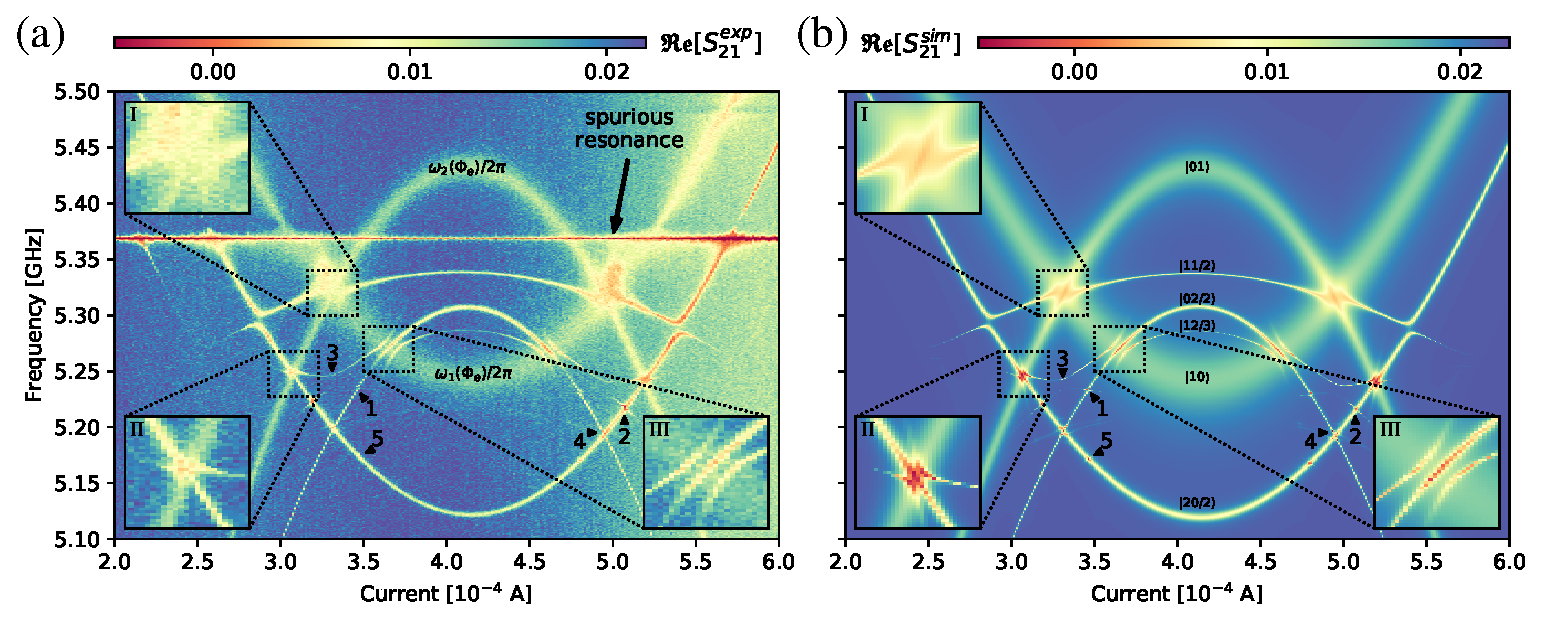
\includegraphics[width=\linewidth]{main_picture}
	
	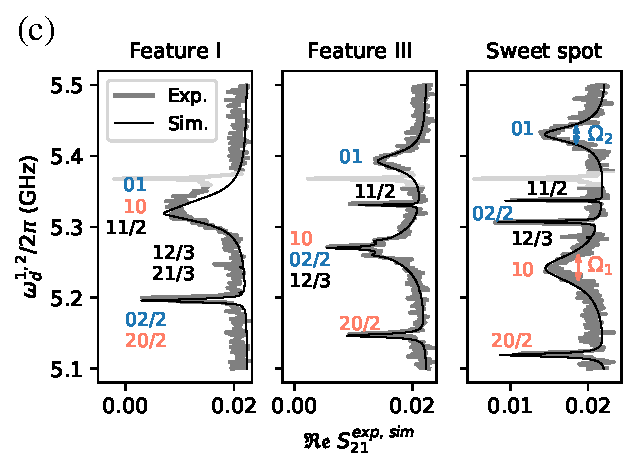
\includegraphics[width=.495\linewidth]{main_picture_slices}
	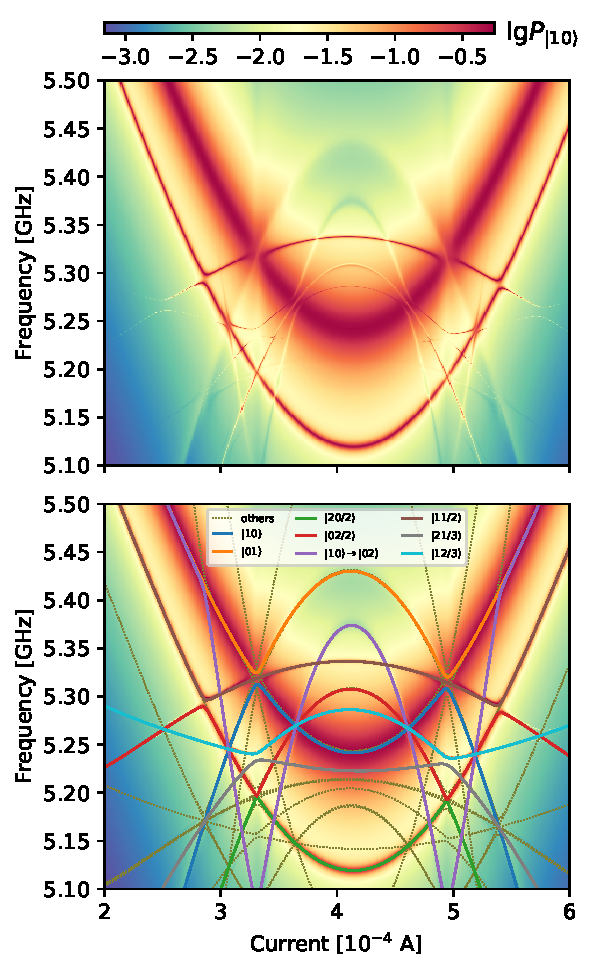
\includegraphics[width=.495\linewidth]{stationary}
	\caption{Two-tone spectroscopy: experiment 
	and numerical modelling. \textbf{(a)} 
	Experimental data. Colour shows the real part 
	of complex transmission  through the sample. 
	Two transmons are aligned as in 
	\autoref{fig:experiment}~(c) and form a 
	symmetric picture. Experimental data contain 
	an additional horizontal line from a 
	parasitic resonance interacting with the 
	readout resonator. Three avoided crossings 
	not predicted by the unperturbed model are 
	shown in insets I, II and III; other 
	pronounced features reproduced by the 
	modelling are shown with Arabic markers (see 
	text for description). \textbf{(b)} Numerical 
	simulation reproducing experimental results 
	with labelled transitions (see Section 
	\ref{sec:analysis} for notation). 
	\textbf{(c)} Slices of (a) and (b) at various 
	currents: 0.365 mA (feature III), 0.411 mA 
	(sweet spot), 0.333 mA (feature I); 
	experiment is gray, simulation is black. 
	Spectral lines where only one SAA is excited 
	are highlighted with the corresponding colour 
	from \autoref{fig:experiment}. Rabi 
	frequencies $\Omega_{1,2}$ may be extracted 
	as FWHM of the spectral lines 10 and 01, 
	respectively. \textbf{(d)} Simulated 
	population of the state $\ket{10}$ ($\lg 
	P_{\ket{10}}$ is shown with colour). Lines 
	show various transition frequencies from the 
	unperturbed Hamiltonian. In the legend, the 
	transitions are labelled near the sweet spot current; if 
	elsewhere any two lines form an avoided 
	crossing, the labels should be swapped after 
	the intersection.}
	\label{fig:two-tone}
\end{figure*}


Experiment was conducted as described in Appendix 
\ref{sec:meas_setup}. We use high-power two-tone 
spectroscopy to probe transitions between 
eigenstates of the SAM; the result is shown in 
\autoref{fig:two-tone}~(a). As one can see, some 
new spectral lines are visible besides the 
fundamental ones that were shown in 
\autoref{fig:experiment}~(c). Their frequency 
also depends on the applied current, and at 
several points they become resonant with each 
other. At three pairs of such resonant points, we 
observe distinct features shown in insets marked 
with Roman numbers. Some secondary details are 
shown with Arabic-numbered markers.

In areas I, II and III, we observe peculiar 
avoided crossings forming triplet transitions. In 
I and II, they are barely visible, however in III 
the splitting is very pronounced. To check 
whether our theoretical model summarized in 
\autoref{eq:master} can reproduce the 
experimental spectrum, we have solved the master 
equation \autoref{eq:master} finding the steady 
states of the system $\hat \rho_{ss}$ and the 
corresponding expected measurement outcomes 
$\mathfrak{Re} \Tr[\hat M \hat \rho_{ss}]$ 
depending on the excitation frequency and 
magnetic flux. The results are shown in 
\autoref{fig:two-tone}~(b) where all the 
experimental details are immediately reproduced 
with just 9 SAM states (i.e., 3 levels for each 
transmon). We have solved \autoref{eq:master} in 
the rotating frame with RWA using 
\autoref{eq:steady} and in the lab frame (using 
the propagator approach \autoref{eq:propagator}) 
and did not find any noticeable difference in the 
results; though, the runtime of the whole 401 by 
401 points simulation was 9 hours without RWA vs. 
3 minutes with RWA. As can be seen from three 
slices of \autoref{fig:two-tone}~(a),(b) in 
\autoref{fig:two-tone}~(c), the numerical results 
are in a good agreement with the experiment (the 
spurious resonance is softened). The parameters 
of model were chosen to match with the 
experimental data.

Remarkably, features I, II and III turn out to be 
impossible to explain using only the unperturbed 
Hamiltonian; we confirm this by numerical 
diagonalization taking the same 9 SAM states as 
in the previous simulation. All possible 
transitions between all resulting eigenlevels of 
the SAM depending on the coil current are shown 
in \autoref{fig:two-tone}~(d) with solid and 
dashed lines. While correctly reproducing, for 
instance, the avoided crossing labelled as 
feature 3 in \autoref{fig:two-tone}~(a), it 
completely misses the Roman-numbered effects. 

So far, we have established the fact that the 
same model SAM yields different spectra depending 
on the presence of the driving, and that the full 
model \autoref{eq:master} agrees well with 
experimental data. To understand the nature of I, 
II and III, we describe \autoref{fig:two-tone} in 
more detail in a separate section below.

\begin{figure*}
	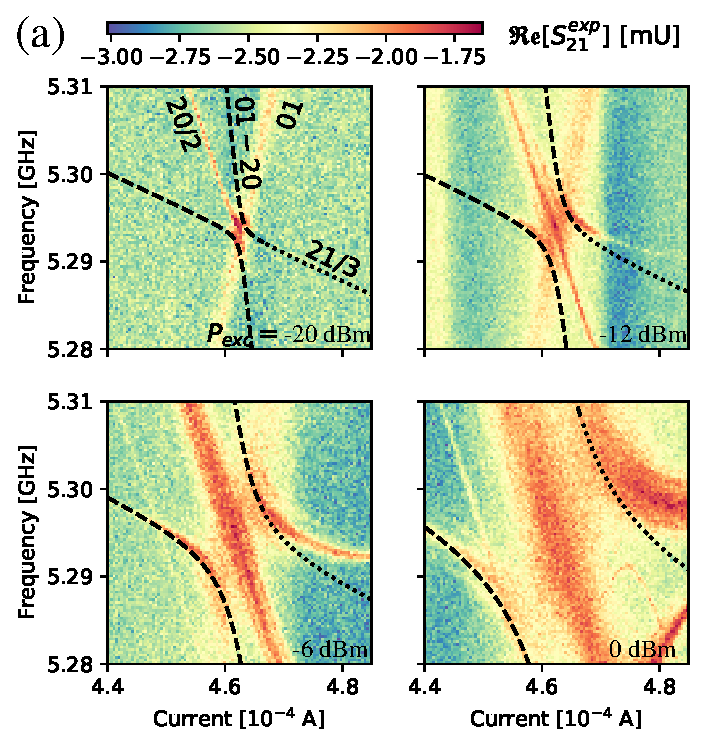
\includegraphics[width=.49\linewidth]{powerscan}
	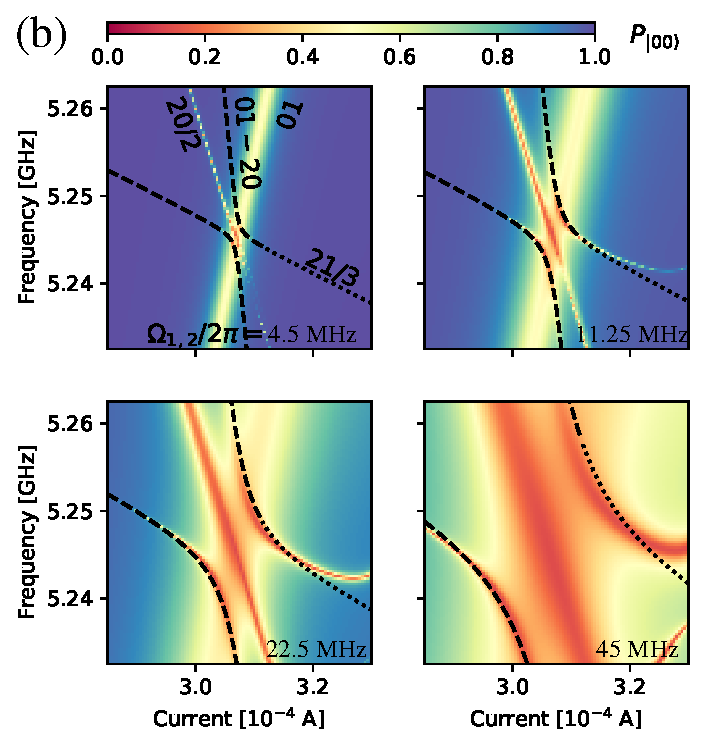
\includegraphics[width=.49\linewidth]{zoom2_picture}
	
	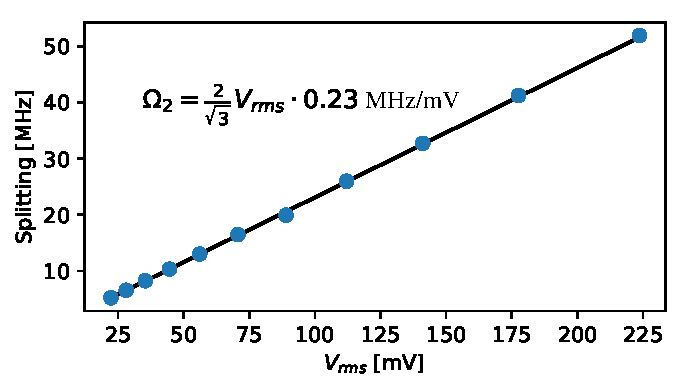
\includegraphics[width=.7\linewidth]{powerscan_1d}
	\caption{Power dependence of feature II: 
	experiment, simulation and analytic model. Dashed are the model curves turning to dotted when the 
	model is not expected to be valid (see 
	Sections \ref{sec:theory} and 
	\ref{sec:münchhausen}); model values for 
	$\Omega_{1,2}$ are the same for both (a) and 
	(b): $\Omega_{1,2}/2\pi=$ 4.5, 11.25, 22.5 
	and 45 MHz. \textbf{(a)} Experiment (second 
	cooldown; the parameters are different to 
	those in \autoref{fig:experiment}). The power 
	of the microwave source is increased from -20 
	to 0 dBm, and the corresponding growth of the 
	splitting and the widths of the spectral 
	lines is observed. \textbf{(b)} Simulation 
	with amplitudes of the driving $\Omega_{1,2}$ 
	equal to the model values; other parameters 
	as in \autoref{fig:two-tone}. Note that now 
	colours show the population of the ground 
	state. \textbf{(c)} Linear dependence of the 
	splitting size on the driving voltage of the 
	microwave source $V_{rms} = 
	\sqrt{10^{P_{exc}/10}\cdot 1 \text{ mW} \cdot 
	50\ \Omega}$, ${\Omega_2}/{V_{rms}} = 0.23\ 
	{\text{MHz}}/{\text{mV}}$. From Section 
	\ref{sec:theory}, the splitting size is 
	$\frac{2\sqrt{3}}{3} \Omega_2$.}
	\label{fig:zoom}
\end{figure*}


\begin{figure*}
	\centering
	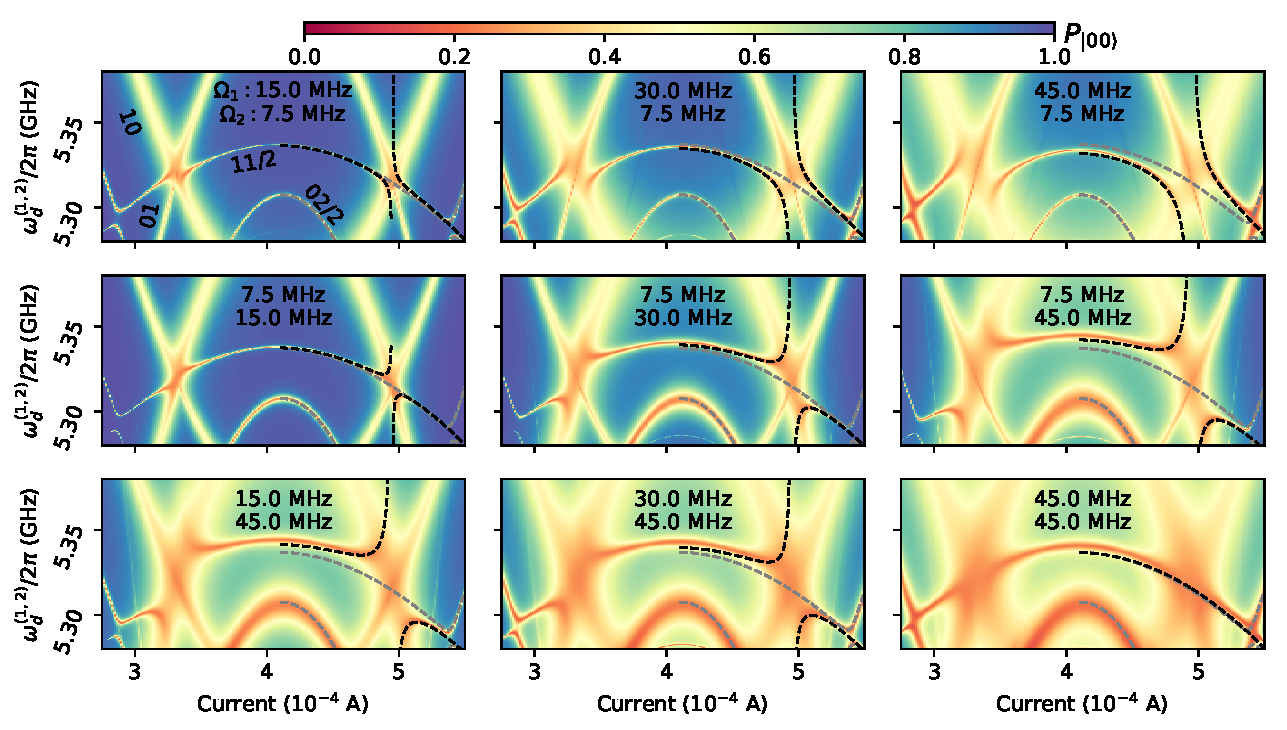
\includegraphics[width=\linewidth]{topological_splittings}
	\caption{Simulated population of the ground 
	state when the transmons are driven at the 
	same frequency but at different amplitudes 
	$\Omega_{1,2}$. In the top row (middle row), 
	$\Omega_{1(2)}$ is increased while 
	$\Omega_{2(1)} = \text{const} \ll 
	\Omega_{1(2)}$; two topologically different 
	types of anticrossings arise depending on 
	which transmon is driven stronger. In the 
	bottom row, we show how the splittings vanish 
	when the weaker driving is increased to match 
	with the stronger one. Gray dashed lines show 
	the solution without driving, in black are 
	the model curves based on Sections 
	\ref{sec:theory} and \ref{sec:münchhausen}.}
	\label{fig:difdrive}
\end{figure*}


\subsection{Analysis of the spectra} 
\label{sec:analysis}

\paragraph{Identification of the spectral lines.} 
Though it is not possible to describe all of the 
experimental features with the unperturbed model, 
we can still use it to identify most of the 
observed transitions as follows. As said above, 
by numerical diagonalization, we calculate the 
unperturbed frequencies of the undriven SAM as 
$\omega_{mn} = (E_n - E_m)/h$ where $n>m,\  
n,m=0..9$. In \autoref{fig:two-tone}~(d), we 
place them over the heatmap data depicting the 
population of $\ket{10}$ optionally dividing 
$\omega_{mn}$ by some integer $n$ to find the 
frequency of an $n$-photon process to find a 
match among the visible lines in the heatmap. 
Since the number of SAM states is finite, we can 
quickly find all such correspondences. 

Next, at the sweet spot, we name the found lines 
as $ij/n$ where $i,j$ denote the final basis 
state $\ket{ij}$ of the SAM after the transition 
from the ground state, and $/n$ is optional for 
an $n$-photon process. We can do that because at 
the sweet spot the transmons are detuned from 
each other, and thus SAM eigenstates are nearly 
factorized (dispersive regime). Using this 
notation, we label lines in 
\autoref{fig:two-tone}~(b),(c), as well. One 
should be careful because for 
\autoref{fig:two-tone}~(d) this notation is valid 
only near the sweet spot before any two lines 
form an avoided crossing. When they do, their 
names should be swapped.
 
Having settled the naming system, we continue to 
analyse the plots. Due to the strong driving, we 
observe several multiphoton transitions besides 
the main lines at $\omega_{(1,2)}(I)/2\pi$ (or 
$01$ and $10$ lines). The ${02/2}$ and ${20/2}$ 
are very commonly found for transmons and lie 
$|\alpha_{(1,2)}|/2$ lower than the main lines 
$\omega_{(1,2)}(I)$. Another two-photon process 
appears as $11/2$ line when two SAAs are excited 
simultaneously. This process is used, for 
example, for doing the bSWAP 
gate\cite{poletto2012entanglement}; in our case, 
it is taking part in formation of feature I. A 
three-photon process $12/3$ is also clearly 
visible just below the $02/2$ line. As we will 
see, processes $12/3$~and~$21/3$ are involved in forming features III and II, respectively. Notably, transitions $11/2$, ${21/3}$ and 
${12/3}$ are forbidden when there is no 
interaction between transmons ($J=0$). Therefore, 
it is expected that all Roman-numbered features 
should only appear with non-vanishing $\hat 
H_{int}$.

When two lines intersect, they may form an 
avoided crossing even for an unperturbed model if 
the corresponding matrix 
element of $\hat H_{int}$ is non-zero. In such 
cases, the SAM becomes inseparable with some of 
the eigenstates becoming superpositions of the 
factorized states. For a two-transmon SAM, such 
points are, for instance, anticrossings between 
${01}$,${10}$ or $ {11} $,$ {02} $($ {20} $) 
visible clearly in \autoref{fig:two-tone}~(d). 
Additionally, marked as feature 3 in 
\autoref{fig:two-tone}, we see an avoided 
crossing between ${12}/3,\ {21}/3$ at the same 
current where ${01}$, ${10}$ intersect.


\paragraph{Analysing features I, II and III.} 
First, we have reproduced the avoided crossing of feature III in an additional numerical simulation taking only 2 levels for the transmon 1 and three levels for 
the transmon 2. Upon this, it has become clear 
that features II and III are actually of 
the same nature and differ only by the ordering 
of the transmons: for II, they appear whence the 
transition ${01}$ intersects with the two-photon 
one ${20/2}$, and for III when ${10}$ intersects ${02/2}$; 
one can see this clearly in 
\autoref{fig:two-tone}~(b).

From \autoref{fig:two-tone}~(d) we conclude that 
avoided crossing in III is between two 
transitions: ${12/3}$ (three-photon transition $\ket{00}\rightarrow\ket{12}$) and ${10} - {02}$ 
($\ket{10}\rightarrow\ket{02}$) which are of the 
same frequency when $\omega_1 = 
\omega_2+\alpha_2/2$. The latter process is depopulating $10$ and it is better discernible in \autoref{fig:two-tone}~(d) 
than in \autoref{fig:two-tone}~(a), (b). For II, the 
opposite is true: ${21/3}$ and ${01} - {20}$ are 
crossing when $\omega_2 = \omega_1+\alpha_1/2$. 
From additional measurements and simulations, we 
find that the splitting depends on the driving 
power; the experimental and simulated results for 
II are shown in colour in \autoref{fig:zoom}~(a), (b), respectively. As one can see, the growth of the splitting with 
increasing power is linear: it is roughly equal 
to the FWHM of the ${01}$ spectral line. To fully 
quantify the shape of this splitting, in Section 
\ref{sec:theory} we derive analytical expressions 
for the dashed curves fitting the spectral lines 
in \autoref{fig:zoom}. In \autoref{fig:zoom}~(c), blue points, we present splitting sizes extracted by fitting of the model to the data as in \autoref{fig:zoom}~(a) for various power values of the microwave generator connected to the excitation waveguide. As one can see from the linear approximation of the points, the splitting indeed is simply proportional to the RMS voltage of the signal. From the model, we expect that the minimal distance between curves in the anticrossing is equal to $\frac{2\sqrt{3}}{3} \Omega_2$; using this relation, we extract the proportionality coefficient between $\Omega_2$ and $V_{rms}$ is around $0.23$ MHz/mV from the linear fit.

In \autoref{fig:difdrive}, we demonstrate a similar power dependence of feature I: increasing drive amplitude on one of the 
transmons while keeping the other one small and 
constant again elicits avoided crossings with the 
proportional size. We  show only the simulation results; an experiment is not possible with our sample because, since we have just a single excitation line, there is 
no way for us to control the driving amplitudes 
$\Omega_{1,2}$ individually. We note that two 
qualitatively different patterns arise depending 
on which of the transmons is driven stronger than 
the other. From this and from the shape of the 
splitting in feature I of 
\autoref{fig:two-tone}~(a), we can infer that 
$\Omega_1/\Omega_2 \approx 2$ there (also 
consistent with the 01, 10 linewidths in 
\autoref{fig:two-tone}~(c)). If in contrast both transmons are driven with equal amplitudes, the avoided crossing vanishes. As can be seen from black dashed lines in \autoref{fig:difdrive}, all these cases are explained well by our analytical model described in detail in Sections \ref{sec:theory} and \ref{sec:münchhausen}.

From all presented observations, we conclude that effects I -- III 
are caused by light dressing. In the case III, the 
first transmon is dressed by a strong resonant 
field; in case II, the second one; finally, in 
case I, both transmons may be dressed at the same 
time. We will discuss these effects in greater 
detail in Sections \ref{sec:theory} and \ref{sec:münchhausen}.

\paragraph{Secondary features.} Using 
\autoref{fig:two-tone}~(d), we can get an insight 
into the features 1 -- 5 as well. 

Feature 1 is a small avoided crossing between 
${02/2}$ and ${21/3}$. It is missing in the 
unperturbed solution and thus is caused by the 
light dressing just as I -- III. Feature 2 is its 
twin: ${12/3}$ and ${20/2}$ intersect there but 
the anticrossing is smaller due to the asymmetry 
of the driving strengths and is not resolved. 

Feature 3 is a large avoided crossing between 
three-photon processes ${12/3}$ and ${21/3}$. It 
is predicted by the unperturbed model, and direct 
diagonalization yields the splitting of 
$\frac{4}{3}J$. A remarkable detail here is that 
the dim lower branch implies the presence of a 
dark state with respect to the driving operator 
in the third order. 

Feature 4 is also explained by the unperturbed 
model and is caused by several spectral lines and 
a pair of avoided crossings near a single point 
(dotted lines in \autoref{fig:two-tone}~(d)). It 
appears at the point where ${02/2}$ intersects 
${20/2}$ and is just barely visible in the 
experimental data because of the noise. 

Feature 5 is located at the intersection between ${20/2}$ 
and ${10} - {02}$, and can be 
found in the experimental data, too. 

In conclusion to this section, we note that when the coupling is turned off ($J=0$) in the simulation, the system does not demonstrate any of the described details. This means that all these effects can only be attributed to the SAM as a whole. 

\subsection{Explaining extra avoided crossings}\label{sec:theory}

Since we had already connected the additional 
avoided crossings with the light dressing, it was 
natural to expect an Autler-Townes-like effect to 
be at the root of the additional spectral lines. 
For a three-level system, the standard A-T effect 
is revised in Appendix \ref{sec:3-level-at}. 
However, in our case the level structure and the 
effect itself are more complicated. 

First of all, since during the spectroscopy we 
apply only a single microwave tone ($\omega_d^1 = 
\omega_d^2$), it has to be 
simultaneously the coupler and the probe
in terms of the standard A-T effect; moreover, the 
probe must be much weaker than the coupler. 
Fortunately, all these conditions are satisfied near feature II(III) when 
$\omega_{\{2,1\}} = 
\omega_{\{1,2\}}+\alpha_{\{1,2\}}/2$  where we 
can simultaneously excite transitions $01 (10)$ 
and $20/2 (02/2)$. Since the two-photon Rabi 
frequency is much smaller than the single-photon 
$\Omega_2$, it is natural to view this two-photon 
excitation as the probing process which does not 
affect the level structure. In contrast, 
single-photon excitation is strong enough to 
dress the system. In other words, in our case the 
A-T coupling operator is $\hat H_{d}^1$ (strong), 
and the probing operator is $\hat H_{d}^2$ (weak 
in the two-photon regime). However, their 
separation in our case is not in frequency, but 
in the Hilbert subspaces they act upon and in the number of participating photons.

For feature I, the simultaneously 
excited transitions are $01,\ 10$ and the 
two-photon $11/2$. In this case, the weak two-photon process is probing transitions in the doubly-dressed SAM. We find that if SAAs are dressed equally, $11/2$ does not form an avoided crossing, and for it to be clearly observed it is required that 
$\Omega_{\{1,2\}} \gg \Omega_{\{2,1\}}$. 

Below, we give the detailed explanation of features II and III, and finally, I.

\begin{figure}
	\centering
	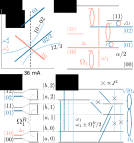
\includegraphics[width=\linewidth]{main_scheme_2}  
	\caption{Explaining feature III. \textbf{(a)} 
	Schematic of the transition frequencies near 
	III (not to scale). Black dashed line shows the 
	current (0.36 mA) where the first transmon 
	(orange) is below the second one (blue) 
	exactly by $\alpha_2/2$ and several 
	transitions become resonant. Here we assume 
	that each transmon is driven at its own 
	frequency. \textbf{(b)} System level 
	structure at the resonant point and the first transmon 
	driving of amplitude $\Omega_1$ 
	(orange ellipses) at a small detuning 
	$\Delta_1$ from $\omega_1$. The second 
	transmon driving is not shown here. Action of 
	$\hat H_{int}$ in RWA is depicted as 
	orange-blue circles. \textbf{(c)} In the 
	frame rotating with $\hat 
	H_{d}^1$, states $\ket{0j},\ket{1j}$ 
	become nearly degenerate ($\omega_1 
	\rightarrow \Delta_1$). Dressing increases this splitting to 
	$\Omega_1^R = \sqrt{\Omega_1^2 + 
	\Delta_1^2}$. \textbf{(d)} Transitions in the 
	dressed system induced by $\hat 
	H_{d}^2$ (coupled level subspaces are shown with blue ellipses). In 
	the left part of the panel, all possible 
	two-photon transitions near $\omega_1$ are 
	depicted: the blue transitions are not 
	shifted in frequency, the light blue ones are shifted 
	by $\pm\Omega^R_1/2$. In the right 
	part, the most contributing trajectories are 
	depicted; gray crosses show transitions that 
	are forbidden without the coupling $J$.}
	\label{fig:main_scheme}
\end{figure}

\begin{figure}
	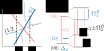
\includegraphics[width=.9\linewidth]{topo_scheme}
	\caption{Explaining feature I. (a) Schematic of the transitions near I. (b) Transitions in the frame rotating with the second transmon with dressing. As will be shown in Section \ref{sec:münchhausen}, in our experiment there can only be one visible transition to the left or to the right from the resonance.}
	\label{fig:featureI}
\end{figure} 

\paragraph{Features II and III.}  

In \autoref{fig:main_scheme}, we elaborate on which transitions
are involved in the A-T-like effect for feature III. 
For simplicity, we will temporarily assume that 
each transmon is driven at its own frequency 
(this assumption will be lifted in the following 
section). For convenience, in 
\autoref{fig:main_scheme}~(a) we schematically 
reproduce the transitions near III where the 
first transmon (orange) is below the second 
(blue), and the resonance point in current is 
shown with a dashed black line. Next, 
\autoref{fig:main_scheme}~(b) demonstrates the 
level structure of the SAM at 0.36 mA. Detuned by 
$\Delta_1$ from $10$, single-photon driving of 
$\hat H_d^1$ is shown with orange ellipses while 
much weaker two-photon $\hat H_d^2$ is not shown 
yet. Since from numerical simulations we know 
that the third level of the first transmon is not 
necessary to observe the splitting, $\ket{20}$ is 
shown transparent, and states $\ket{21},\ 
\ket{22}$ are not shown.

The next step is to view the system in the frame 
rotating with the first transmon 
(\autoref{fig:main_scheme}~(c)) and then move to 
the  dressed picture similarly to Appendix 
\ref{sec:3-level-at}. Now, the first transmon 
splitting equals $\Omega_{1}^R = 
\sqrt{\Omega_1^2+\Delta_1^2}$, and its new 
eigenstates (dressed states) are denoted 
$\ket{a}$ and $\ket{b}$. Meanwhile, the second 
transmon energies stay the same.


Finally, in \autoref{fig:main_scheme}~(d) we demonstrate possible two-photon transitions between the dressed states induced by the second transmon driving $\hat H_{d}^2$. In the left part of the panel, one can find the unmodified two-photon transition $02/2$ at $\omega_1$ and two sidebands at $\omega_1 \pm \Omega_1^R/2$. This picture finally explains the observed triplet transition of feature III. The right part describes the mechanism of these two-photon processes through virtual excitations of the intermediate states. From here it becomes obvious that without the transmon-transmon interaction the sideband transitions are forbidden due the selection rule: $\bra{a,j}\hat{\mathbbm{1}}\otimes \hat n_2 \ket{b, j+1} = 0$ since $\braket{a}{b} = 0$. However, we will show that they become allowed in the second order in $J$ when the coupling is turned on.

Now, we will repeat this reasoning using a 
quantitative mathematical model. We start from 
the initial Hamiltonian \autoref{Hsystem}. To 
move to the rotating frame with 
\autoref{eq:rotation} and apply the RWA, we use 
the following operator:
\begin{equation}
R = \exp[-it \omega_d^1 
(b^{\dagger}b+c^{\dagger}c)].
\end{equation}  
Note that now we rotate both transmon subspaces simultaneously in contrast to what is shown in \autoref{fig:main_scheme} because below it will be convenient to have time-independent $\hat H_{int}$. Now,
\begin{equation}
\begin{aligned}
\omega_{(1,2)} &\rightarrow \Delta_{(1,2)} = \omega_{(1,2)} - \omega_d^{1},\\
\hat H_{int} &\rightarrow  \hbar J \left[\hat \sigma_+ \hat c + \hat \sigma_-\hat c^\dag \right],\\
\hat H_{d}^1 &\rightarrow \frac{\hbar \Omega_1}{2} \hat \sigma_x,\ 
\hat H_{d}^2 \rightarrow \frac{\hbar \Omega_2}{2}(\hat c e^{i\delta t}  + \hat c^\dag e^{-i\delta t}),
\end{aligned}
\end{equation}
where $\delta = \omega_{d}^2 - \omega_{d}^1$.

Since $\hat H_{d}^1$ is now time-independent, we can move to the dressed basis by applying a transformation $\hat S$ which diagonalizes the first transmon. After that, the Hamiltonian may be split into three parts
\begin{equation}
\begin{aligned}
\hat H^{D}/\hbar &= \left[\frac{\Delta_1}{2} 
\hat{\mathbbm{1}}-\frac{\Omega_1^R}{2}\hat 
\sigma_z\right] + \Delta_2 \hat b^{\dagger}\hat b 
+\frac{1}{2}\alpha_2 \hat b^{\dagger}\hat b(\hat 
b^{\dagger}\hat b-1),\\
\hat V_J &= \hat S^\dag \hat H_{int}\hat S,\\
\hat V_t &= \hat S^\dag \hat H_{d}^{2} \hat S \equiv \hat H_{d}^{2}.
\end{aligned}
\end{equation}
The first part is diagonal, and the remaining two 
will be treated as perturbations. To simplify 
further calculations, we consider the point where 
$\Delta_1 = 0$ and $\Delta_2 = - \alpha_2/2$. In 
these conditions, $H^D$ becomes degenerate as can 
be seen in \autoref{eq:ham_matrix} of Appendix 
\ref{sec:dpt}. Using the degenerate perturbation 
theory for $\hat V_J$ summarized therein, we find 
the first-order corrected wave functions of $\hat 
H^D + \hat V_J$, labelled $\ket{k},\ k=1..6$. 

The time-dependent perturbation theory that we use to calculate the transition rates of the two-photon processes stimulated by $\hat V_t$ is reviewed in Appendix \ref{sec:2pp}. Using the corrected eigenstates $\ket{k}$ and neglecting small terms, we obtain the following expressions for the transition rates per unit time\cite{faisal2013theory}:
\begin{equation}
\begin{aligned}
R^{(2)}_{1\rightarrow 6} &\approx 2\pi\Omega_2^4 
\frac{18 J^4 \left(2 \alpha + 
\text{$\Omega_1$}\right)^2}{\alpha 
^{6}\Omega_1^2},\\
R^{(2)}_{2\rightarrow 5} &\approx 2\pi\Omega_2^4 
\frac{18 J^4 \left(2 \alpha - \text{$\Omega_1
		$}\right)^2}{\alpha ^{6}\Omega_1^2},
\end{aligned}\label{eq:rates}
\end{equation}
when $\alpha \gg \Omega_1, \Omega_2, J$ which is 
true for our setup. From \autoref{eq:rates} 
follows that the sideband transitions are 
prohibited without the interaction in the SAM 
$(J=0)$, and the extra avoided crossings will not 
be observed.

\paragraph{Feature I.} Finally, we discuss the 
last Roman-numbered effect. It is illustrated in 
\autoref{fig:featureI} for the case when 
$\Omega_2 \gg \Omega_1$: the second transmon is 
dressed, and the splitting has the shape shown in 
\autoref{fig:featureI}~(a). For the opposite case 
($\Omega_1 \gg \Omega_2$), the logic is the same. 

As one can see from \autoref{fig:difdrive}, only the two-photon transition $11/2$ is affected and deviates from unperturbed spectrum when approaching the 01-10 intersection while the other spectral lines are not moving. Similarly to II and III, in the frame rotating with the second transmon it tuns into two different single-photon transitions for $\hat H_d^1$ located at $\omega_1 \pm \Omega_2^R$, see \autoref{fig:featureI}~(b). We will show below that in the experiment with a single excitation frequency, it is not possible to observe both transitions simultaneously; this is clearly visible in \autoref{fig:difdrive}. Instead, we observe one line to the left and the other to the right from the 01-10 intersection.




\subsection{Self-consistent equations for the avoided crossings}
\label{sec:münchhausen}

Before, we have assumed that the transmons are driven independently at two different frequencies. In this section, we will employ the same model from \autoref{fig:main_scheme} to explain the experimentally observed splittings when only a single frequency $\omega_d$ is sent at the SAM. 

\paragraph{Features II, III.} We start again with feature III. As shown in 
\autoref{fig:main_scheme}~(d), the sideband 
transitions are formed by two-photon processes 
with $\hat H_d^2$. On the other hand, we know from 
the unperturbed solution that in the laboratory 
frame the two transitions forming the avoided 
crossing are $10 - 02$ (one-photon) and $12/3$ 
(three-photon). This means that there should be a 
smooth transformation between these 1-, 2- and 3-photon 
processes when the system approaches the resonant 
point where $\alpha_2 + 2 \omega_{2} = 2\omega_1$. Let us consider hypothetical two-photon transitions $(10 
- 02)/2$ and $12/2$. In the frame rotating with 
the first transmon like in 
\autoref{fig:main_scheme}~(c) when $\Omega_1$ = 
0, their 
frequencies are
\begin{equation}
\begin{aligned}
\omega_{(10-02)/2} &= (\alpha_2 + 2 \omega_{2} - \Delta_1)/2,\\
 \omega_{12/2} &= (\alpha_2 + 2 \omega_{2} + \Delta_1)/2.
\end{aligned}
\label{eq:two-photon_lab}
\end{equation}
When the first transmon becomes dressed by $\Omega_1 \neq 0$, its splitting $\Delta_1$ changes to $\Omega^R_1 =\sqrt{\Omega_{1}^2 + \left(\omega_{1} - \omega_{d}\right)^{2}}$. Substituting this new splitting into the equations above we find that $\omega_{(10-02)/2}$ and $\omega_{12/2}$ are exactly equal to the two-photon sideband frequencies $\omega_1 \pm \Omega_1^R/2$ established in the previous section. Therefore, it is logical to use them to model the splitting behaviour beyond the resonant point.

Since we are simultaneously dressing the states by $\hat H_d^1$ and probing two-photon transitions between them with $\hat H_d^2$ at $\omega_d$, self-consistent equations have to be solved to find at which $\omega_d$ the sideband spectral lines will appear
\begin{equation}
\begin{aligned}
\omega_{(10-02)/2} &= \omega_d,\\
\omega_{12/2} &= \omega_d.
\end{aligned}
\label{eq:two-photon}
\end{equation}

When $\Omega_1 = 0$, these equations yield indentical pairs of solutions due to the properties of the modulus $|\omega_1 - \omega_d|$. Substituting \autoref{eq:two-photon} into \autoref{eq:two-photon_lab}, we obtain the frequencies and identify them as the three-photon and single-photon transition frequencies in the laboratory frame:
\begin{equation}
\omega_d = \begin{cases} \frac{\alpha_2}{3} + \frac{2 \omega_{2}}{3} + \frac{\omega_{1}}{3}, \\ \alpha_2 + 2 \omega_{2} - \omega_{1}.\end{cases}
\end{equation}
When $\Omega_1 \neq 0$, we obtain the following solutions:
\begin{equation}
\omega_d = \frac{2 \alpha_2}{3} + \frac{4 \omega_{2}}{3} - \frac{\omega_{1}}{3} \pm \frac{\sqrt{3 \Omega_{1}^{2} + \left( \alpha_2 + 2 (\omega_{2} - \omega_{1})\right)^{2}}}{3}.
\label{eq:splitting_model}
\end{equation}
The minimal splitting between these lines is 
found at the resonant point and equals $\frac{2 
\sqrt{3}}{{3}} \Omega_1$. All these calculations 
can be repeated exactly for the feature II by 
swapping the transmons; in that case, the 
splitting will be $\frac{2 \sqrt{3}}{{3}} 
\Omega_2$.

We find excellent agreement between this self-consistent analytical model \autoref{eq:splitting_model} and 
both the experimental and simulated data as can 
be seen in \autoref{fig:zoom}. To plot the model 
curves we have fitted the 
$\omega_{(1,2)}(\Phi_e)$ transitions with simple 
linear functions and substituted them in 
\autoref{eq:splitting_model}; $\alpha_1$ is known 
from spectroscopy. The only free parameter left 
was $\Omega_2$. We have repeated this 
approximation for a range of microwave powers to 
confirm the linear dependence of the splitting on 
excitation amplitude (see \autoref{fig:zoom}~(c)).

The upper branch of the fitted anticrossing is expected to deviate from the model (see dashed curves in \autoref{fig:zoom}) because of the avoided crossing marked as the secondary feature 3 which was not incorporated in the simple linear model. The small discrepancy between the experimental and simulated data in the upper branch is caused by a slight elevation of the lower sweet spot of the first transmon moving the avoided crossing 3 closer to the feature II; however, it is not important for our reasoning.	


\paragraph{Feature I.} Feature I may be explained using the same dressing model. Looking at \autoref{fig:featureI} for the case $\Omega_2 \gg \Omega_1$, we can write another pair of self-consistent equations:
\begin{equation}
\omega_{1} \pm \Omega_2^R = \omega_d.
\end{equation}
Due to the fact that $\Omega_2^R = \sqrt{\Omega_2^2 + (\omega_2 - \omega_d)^2}$, this system has a single solution:
\begin{equation}
\omega_d = \frac{\omega_1 + \omega_2}{2} - \frac{ \Omega_{2}^{2}}{2 \left(\omega_{1} - \omega_{2}\right)},
\label{eq:topo_1}
\end{equation}
which gives back the frequency of $11/2$ in the laboratory frame when $\Omega_2$ is zero. When $\Omega_2$ is non-zero, the solution near the point $\omega_1 \approx \omega_2$ is a hyperbolic curve, which agrees well with the numerical simulation. However, in reality we do not observe the asymptotically vertical parts of this model since it becomes invalid when $|\omega_1 - \omega_2| \leq J$ due to the finite coupling $J$ between the transmons. Since they never reach each other in frequency, the denominator in \eqref{eq:topo_1} is limited from below and there is no divergence.

When $\Omega_1 \gg \Omega_2$, besides the 
replacement $\Omega_2 \rightarrow \Omega_1$, 
\autoref{eq:topo_1} changes the sign:
\begin{equation}
\omega_d = \frac{\omega_1 + \omega_2}{2} + \frac{ \Omega_{1}^{2}}{2 \left(\omega_{1} - \omega_{2}\right)},
\label{eq:topo_1_inv}
\end{equation}
yielding the reversed shape of the splitting.

Continuing this logic, we can write down the resonance condition in the doubly-rotating frame when both transmons are dressed simultaneously:
\begin{equation}
\Omega_1^R \pm \Omega_2^R = 0.
\label{eq:zero-photon}
\end{equation}
Solving it for $\omega_d$, we obtain the 
generalization of \autoref{eq:topo_1} and 
\autoref{eq:topo_1_inv}:
\begin{equation}
\omega_d = \frac{\omega_{1} + \omega_{2}}{2} + \frac{\Omega_{1}^{2} - \Omega_{2}^{2}}{ 2\left(\omega_{1} - \omega_{2}\right)}
\label{eq:topo_comm}
\end{equation}

\autoref{eq:topo_comm} is used to plot the black 
dashed curves in \autoref{fig:difdrive} taking 
the $\Omega_{1,2}$ values from the simulation 
parameters shown therein. The frequencies 
$\omega_{1,2}$ are extracted from the fits to the 
visible spectral lines. We again find good agreement 
between the model and the simulated data.


\section{Discussion}

We have performed spectroscopy measurements of an 
isolated diatomic superconducting artificial 
molecule (SAM) in a regime of strong interaction 
with classical light. Using joint dispersive 
readout to directly access population of the SAM 
eigenstates, we have located several anomalies in 
the spectral data that were impossible to explain 
using the unperturbed model of the system. By 
using extensive numerical modelling explicitly 
including the interaction with light, we have 
reproduced the experimentally discovered effects 
and attributed them to an altered version of the 
well-known Autler-Townes effect.

In the standard A-T effect, the coupler and the 
probe lasers are separated both in frequency and power. 
In our case, there is only a single spectroscopic 
tone interacting with the system; therefore, 
it has to be both the coupler tone and the probe 
tone at the same time. However, since there are 
two components in the driving operator (one for 
each transmon), the separation between the 
coupler and the probe occurs in the Hilbert space and in the number of photons involved 
rather than in frequency and amplitude. The 
effectively weak driving limit for the probe part is 
achieved when it stimulates a two-photon 
transition while the coupler part is resonant 
with a single-photon one being strong enough to dress the 
system. We have built self-consistent models in 
rotating frame to 
model the experimental splittings induced by the 
same field that probes them, and found a good 
agreement between the model, the experiment, and 
the numerical simulation. Interestingly, no new spectral lines appear in this 
more complex case. Instead, for example, spectral 
lines $12/3$ (three-photon) and $10-02$ (single 
photon) morph to an additional avoided crossing of a 
non-standard size of $\frac{2\sqrt{3}}{3} 
\Omega_1$.

Another interesting effect occurs when both 
components of the driving operator are in the 
single-photon regime. Now, both transmons are 
dressed and probed simultaneously. In this case, 
the $11/2$ transition is split at the resonance 
into a hyperbolic curve, never forming a doublet 
in frequency. Moreover, its shape and visibility 
depends qualitatively on the relation between the driving 
amplitudes; for instant, if they are equal, it disappears 
completely. In our sample, we have a fixed ratio 
of approximately 2 between $\Omega_1$ and 
$\Omega_2$ which still allows us to distinguish the 
splitting experimentally. Notably, the frequency of $11/2$ transition far 
from resonance is also changed noticeably with 
changing power, which means that a fast bSWAP 
gate should be performed at a different frequency 
than the unperturbed model predicts. 

Interestingly, the self-consistent models for the 
observed effects are implying that multi-photon 
processes may smoothly change their order. For 
example, for features II and III, we observe a 
continuous transformation of a three-photon and a 
single-photon processes to the second order in 
\autoref{eq:two-photon}, and of a two-photon 
transition to a zero-photon in 
\autoref{eq:zero-photon}.

In overall, irradiating an individual diatomic artificial molecule with intense light calls forth a plethora of effects which can not be directly observed in natural systems and extend the validity of the well-known light-dressing models. Relative ease in attaining powers that cause multiphoton transitions promises even more complex dynamics in multi-atom systems. We are looking forward to investigating strong interaction with light in larger artificial structures such as one-dimensional and two dimensional chains and arrays of superconducting artificial atoms.

\section{Acknowledgements}

We want to thank our parents and our cat Coconut. Also FPI grant

\appendix

\section{Standard Autler-Townes effect for a three-level $\Xi$ atom} \label{sec:3-level-at}

The underlying cause of the A-T effect is the dressing of the atomic levels by strong EM radiation. There are two equivalent mathematical models for it: the light may be classical or quantized.

\begin{figure}[b]	
	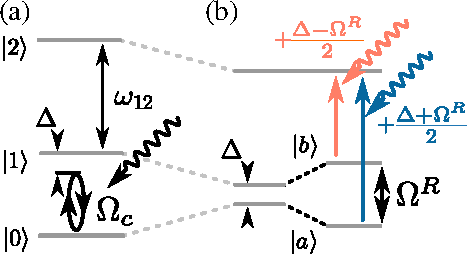
\includegraphics[width=\linewidth]{intro_scheme}
	\caption{Illustrating the A-T splitting by  the classical driving in the rotating frame ($\hbar=1$ here). \textbf{(a)} A three-level system is driven strongly by a ``coupler'' tone of amplitude $\Omega$ at frequency $\omega_{01}-\Delta$ which induces Rabi oscillations between $\ket{0}$ and $\ket{1}$ at the generalized Rabi frequency $\Omega_R = \sqrt{\Omega^2 + \Delta^2}$. \textbf{(b)} Moving to the frame rotating with the drive, we effectively change the $\ket{0}\rightarrow \ket{1}$ transition frequency to $\Delta$. However, when the RWA is applied and Hamiltonian is re-diagonalized, the splitting between two lowest levels (dressed states $\ket{a}$ and $\ket{b}$) becomes $\Omega^R$. Now, the experimenter may observe a doublet transition from these levels to the state $\ket{2}$ at frequencies $\omega_{12}+(\Delta \pm \Omega^R)/2$.} 
	\label{fig:at-standard}
\end{figure}

\paragraph{Classical derivation.} In the classical case, the mathematical description goes as follows. At first, there is a three-level system which is driven by a strong radiation with an amplitude $\Omega_1$ at a frequency detuned by $\Delta$ from the $\ket{0}\rightarrow \ket{1}$ transition with a frequency $\omega_{01}$ (the \textit{coupler} tone). Additionally, we have a weak probe radiation at a frequency $\omega_{p}$ and with an amplitude $\Omega_2$ between $\ket{1}$ and $\ket{2}$ (the \textit{probe} tone). This step is illustrated in \autoref{fig:at-standard}~(a). The Hamiltonian for such system is as follows:

\begin{equation*}
\hat H^c_0/\hbar = \left[\begin{matrix}
0 & \Omega_{1} \cos{\left(\omega_{01}- \Delta \right)t} & 0\\
\Omega_{1} \cos{\left(\omega_{01} - \Delta \right)t}   & \omega_{01} &\Omega_{2} \cos\omega_p t  \\
0 & \Omega_{2} \cos{\omega_p t}  & \omega_{02}\end{matrix}\right].
\end{equation*}

Next, we move to the rotating frame by using an operator
\[
\hat R = \left[\begin{matrix} 
1 & 0 & 0\\0 & e^{- i t \left(\omega_{01}- \Delta\right)} & 0\\0 & 0 & e^{- i t \left(\omega_{01}- \Delta\right)}\end{matrix}\right].
\]
Note here that level $\ket{2}$ is also rotated: this is convenient to preserve the frequency of the driving term with $\Omega_2$. The new Hamiltonian should be calculated as follows: $\hat H_1 = \hat R^\dag \hat H_0 \hat R - i \hat{R}^\dag \partial_t  \hat R$. The level structure without driving  is shown in the left part of \autoref{fig:at-standard}~(b). Applying the RWA, we obtain:
\begin{equation*}
\hat H^c_1/\hbar = \left[\begin{matrix}0 &\Omega_{1}/2 & 0\\\Omega_{1}/2 & \Delta & \Omega_{2} e^{i t \omega_p}/2\\0 & \Omega_{2} e^{-i t \omega_p}/2 & \omega_{02} - \omega_{01}+\Delta \end{matrix}\right].
\end{equation*}

Next, moving to the basis where the upper left 2x2 corner is diagonal (the right part of \autoref{fig:at-standard}~(b)), we obtain:

\begin{equation*}
\hat H^c_3/\hbar = \left[\begin{matrix} 
\frac{\Delta}{2} - \frac{\sqrt{\Delta^{2} + \Omega_{1}^{2}}}{2} & 
0 &
\frac{\Omega_{2} e^{i t \omega_{p}}}{2}\sin(\theta)
\\
0 & 
\frac{\Delta}{2} + \frac{\sqrt{\Delta^{2} + \Omega_{1}^{2}}}{2} & 
\frac{\Omega_{2} e^ {i t \omega_p}}{2}\cos(\theta)
\\
\frac{\Omega_{2} e^{-i t \omega_{p}} }{2}\sin(\theta) & 
\frac{\Omega_{2} e^{-i t \omega_{p}}}{2} \cos(\theta) & 
\omega_{12} +\Delta 
\end{matrix}\right].
\end{equation*}

One may see that now resonant conditions for the probe drive are $\omega_p = \omega_{12} + \dfrac{(\Delta \pm \Omega^R)}{2}$, where $\Omega^R = \sqrt{\Omega_1^2 + \Delta^2}$, $\omega_{12} = \omega_{02}- \omega_{01}$, and its amplitude is renormalized by an angle $\theta,\ \tan 2\theta = -\frac{\Omega_1}{\Delta}$.


\paragraph{Quantum derivation.} For the fully quantum interpretation, we model the incident radiation at the frequency $\omega_{01}-\Delta$ as a single-mode quantum oscillator which is coupled to the system. The Hamiltonian for this model will be as follows:
\[
\begin{split}
\hat H^q_0/\hbar = \omega_{01} \ket{1}\bra{1} + \omega_{02} \ket{2}\bra{2} + (\omega_{01}-\Delta) \hat a^\dag \hat a + \\\ g (\hat a^\dag + \hat a)\otimes (\ket{1}\bra{0}+\ket{0}\bra{1}),
\end{split}
\]
where $g$ is the coupling strength and $a$ is the photon annihilation operator. After moving to the rotating frame with $\hat R = \exp[i t (\omega_{01}-\Delta)(\hat a^\dag \hat a + \ket{1}\bra{1}+\ket{2}\bra{2})]$ and applying the RWA, the Hamiltonian transforms into
\begin{equation}
\begin{split}
\hat H^q_1/\hbar = \Delta \ket{1}\bra{1} + (\omega_{12}+\Delta) \ket{2}\bra{2} + \\\ g \left[\hat a^\dag \otimes \ket{0}\bra{1} + \hat a \otimes \ket{1}\bra{0}\right].
\end{split}
\end{equation}
If we presume that the resonator is in a coherent state $\ket{\alpha e^{-it(\omega_{01}-\Delta)}}$ with $\langle N\rangle = \alpha^2$ photons and average $\hat H_1^q$ over the resonator subspace, we from the interaction term will obtain again the classical driving strength $\Omega_1 = 2 \sqrt{\langle N \rangle} g$ in correspondence with the classical driving case. Similarly, the energy levels $\ket{1, N-1}$ and $\ket{0, N}$ become mixed due to the coupling, and their splitting changes from $\hbar\Delta$ to $\hbar\Omega_R = \hbar\sqrt{\Omega_1+\Delta}$. The following steps completely reproduce the classical case if we add the probe tone $\Omega_2$ in the last equation.

\section{Degenerate perturbation theory}
\label{sec:dpt}

Since the Hamiltonian in the dressed basis is a 
useful illustration for 
\autoref{fig:main_scheme}, we provide it below in 
\autoref{eq:ham_matrix} for the case $\Delta_1 = 
0$, $\delta = \omega_d^2 - 	\omega_d^1 = 
\omega_d^2 - \omega_1$. The degeneracy between 
states $\ket{a, 0}, \ket{a,2}$ and $\ket{b, 0}, 
\ket{b,2}$ occurs only in the resonant case 
$2\Delta_2   + \alpha_2 = 0$ meaning that the 
second transmon frame is rotated at its 
two-photon transition frequency. In this 
situation, its single-photon subspace is detuned 
by $-\alpha/2$.



Note that $\hat V_J = \hat S^T \hat H_{int} \hat 
S$ that we treat as perturbation now has an sub- 
and super-diagonal block form and couples all the 
states $\ket{a, j}, \ket{a,j+1}$ and $\ket{b, j}, 
\ket{b,j+1}$.


The choice of zero-order state vectors $\ket{N^0}$ from a degenerate subspace is arbitrary because any linear combination of basis vectors $\ket{n}$ from this subspace will satisfy the unperturbed Schrödinger equation. However, if we demand the \textit{change} of $\ket{N^0}$ to be small under the perturbation $\hat V_J$, they become determined and are given by diagonalization of $\hat V_J$ in the degenerate subspace. Unfortunately, $\hat V_J$ is zero in both our subspaces, so technically any choice of zero-order states will diagonalize $\hat V_J$. In other words, the degeneracy is not lifted in the first-order, and thus we have diagonalize the matrix\cite{landau2013quantum}
\begin{equation}
	M_{nn'} = \sum\limits_{m}\frac{V_{ nm}V_{mn^\prime}}{E_n-E_m}.
\end{equation}
Here, $\ket{n}$ and $\ket{n'}$ are the basis 
states from the degenerate subspace with energy 
$E_n$, and $V_{mn} = \bra{m} \hat  V_J \ket{n}$. 
The sum is over all other zero-order states 
$\ket{m}$ outside the degenerate subspace.



\renewcommand{\kbldelim}{[}% Left delimiter
\renewcommand{\kbrdelim}{]}% Right delimiter
\begin{widetext}
	\begin{equation}
	\hat H^D + \hat V_J + \hat V_t  = 
	\kbordermatrix{
		&\ket{a,0} & \ket{b,0} & \ket{a,1} & 
		\ket{b,1} & \ket{a,2} & \ket{b,2} \\
		\ket{a,0}& -\frac{\Omega_1}{2} & 0 & 
		\frac{\Omega_{2}e^{i \text{$\delta$} 
		t}}{2} -\frac{J}{2} & \frac{J}{2} & 0 & 0 
		\\
		\ket{b,0} & 0 & \frac{\Omega_1}{2} & 
		-\frac{J}{2} & \frac{\Omega_2 e^{i \delta 
		t}}{2} + \frac{J}{2} & 0 & 0 \\
		\ket{a,1} &\frac{\Omega_2 e^{-i 
		\text{$\delta$} t} }{2}  - \frac{J}{2} & 
		-\frac{J}{2} & - \frac{\alpha}{2} - 
		\frac{\Omega_1}{2}&
		0 & \frac{\text{$\Omega_2$} e^{i 
		\text{$\delta$} t}}{\sqrt{2}} 
		-\frac{J}{\sqrt2} & \frac{J}{\sqrt2} \\
		\ket{b,1} & \frac{J}{2} & 
		\frac{\text{$\Omega_2$} e^{-i 
		\text{$\delta $} t}}{2} +\frac{J}{2} & 0 
		& - \frac{\alpha}{2} + \frac{\Omega_1}{2} 
		& -\frac{J}{\sqrt 2} & 
		\frac{\text{$\Omega_2$} e^{i \text{$\delta
					$} t}}{\sqrt 2} + 
					\frac{J}{\sqrt 2} \\
		\ket{a,2} & 0 & 0 & \frac{\Omega_2 e^{-i 
		\delta t}}{2} - \frac{J}{\sqrt 2} & 
		-\frac{J}{\sqrt 2} &
		-\frac{\Omega_{1}}{2} & 0 \\
		\ket{b,2} & 0 & 0 & \frac{J}{\sqrt 2} & 
		\frac{\text{$\Omega_2$} e^{-i 
		\text{$\delta $} t}}{\sqrt 2} + 
		\frac{J}{\sqrt 2} & 0 & 
		\frac{\Omega_{1}}{2}\\
	}
	\label{eq:ham_matrix}
	\end{equation}
\end{widetext}

For example, in our case for one of the degenerate subspaces ($E_n^0 = -\Omega_1/2,\ \hat V = \hat V_J$) we obtain the following matrix:
\renewcommand{\kbldelim}{[}% Left delimiter
\renewcommand{\kbrdelim}{]}% Right delimiter
\begin{equation}
	M_{15} =\kbordermatrix{&\ket{a,0} & \ket{a, 2}\\
	\ket{a,0}&\frac{J^{2} \left(\Omega_{1} - \alpha\right)}{\alpha \left(2 \Omega_{1} - \alpha\right)} &
	\frac{\sqrt{2} J^{2} \Omega_{1}}{\alpha \left(2 \Omega_{1} - \alpha\right)}\\
	\ket{a, 2}&\frac{\sqrt{2} J^{2} \Omega_{1}}{\alpha \left(2 \Omega_{1} - \alpha\right)} &
	\frac{2 J^{2} \left(\Omega_{1} - \alpha\right)}{\alpha \left(2 \Omega_{1} - \alpha\right)}}.
\end{equation}
The normalized eigenvectors 
\begin{equation}
\ket{N} = C_n \ket{n} + C_{n'}\ket{n'}, 
\ket{N'} = C'_{n}\ket{n} + C'_{n'}\ket{n'}
\end{equation}
of the matrix are the desired zero-order superpositions. Next, we first-order correct them as usual:
\begin{equation}
	\ket{N}+\ket{N^{1}} = \sum_{j=n,n'} C_{j}\ket{j} + \sum_{j\ne n, n'}\ket{j}\frac{\bra{j}\hat V\ket{N}}{E_n-E_j}.
\end{equation}

Similarly, the first-order corrections for a non-degenerate state are
\begin{equation}
	\ket{m^1} = \sum_{j\ne m}\ket{m}\frac{\bra{j}\hat V\ket{m}}{E_m-E_j}.
\end{equation}

\section{Transition rates of the two-photon process}\label{sec:2pp}
We will employ the time-dependent perturbation theory that gives analytical expressions for the transition rates for single and multi-photon processes\cite{faisal2013theory}.

Let's consider a time-dependent perturbation $\hat V(t) = \hat V \cos{\omega_d t}$ to the unperturbed Hamiltonian $\hat H$. In the interaction picture, the Schrödinger equation looks as 
$$
i\hbar \partial_t{\psi(t)} = \hat {V_I}(t)\psi(t),
$$ 
where 
$$
\hat {V}_I(t) = e^{\frac{it}{\hbar}\hat H}\hat V(t)e^{-\frac{it}{\hbar}\hat H}.
$$
The eigenstate of $\hat H$ with eigenvalue $E_j$ will be denoted as $\ket{j}$, whence it follows that
$$
\bra{j}\hat{V}_I(t)\ket{i} = e^{i\omega_{ij} t}\bra{j}\hat V(t)\ket{i},
$$
where $\hbar \omega_{ij} = E_j - E_i$. Formally, we can write down the solution of the Schrödinger equation in the interaction picture corresponding to the initial state $\ket{i}$ as
\begin{equation}\label{forpsi}
	\ket{\psi_i(t)}=\ket{i} - i \int_{-\infty}^{t} d\tau_1 \hat{V}_I(\tau_1)\ket{{\psi_i}(\tau_1)}.
\end{equation} 
Solving \autoref{forpsi} by simple iterations 
gives the series solution for it:
\begin{align}
	U(t,-\infty) &= 1 + \sum_{n} U^{(n)}(t,-\infty),\\
	U^{(n)}(t,-\infty) &= -i^n \int\limits_{-\infty}^{t}d \tau_1\hat V_I(\tau_1)...\int\limits_{-\infty}^{\tau_{n-1}}d \tau_n\hat{V}_I(\tau_n),
\end{align}
where $U(t,-\infty)$ is the evolution operator. For a weak perturbation, this series may be truncated at a finite term $n$, and the $n^{\text{th}}$ order transition amplitude $\bra{f}U^{(n)}(t,-\infty)\ket{i}$ can be evaluated:
\begin{equation}
	\begin{aligned}
	\bra{f}U^{(1)}(t,-\infty)\ket{i}&=-i\int\limits_{-\infty}^{t}d\tau_1\hat{V}_I(\tau_1)\\ &=-i\frac{\Omega}{2}\big[\int\limits_{-\infty}^{t}d\tau_1 e^{i(\omega_{if}-\omega_d)\tau_1}\bra{f}\hat{B}\ket{i}+\\
	&\quad\quad\quad\quad\int\limits_{-\infty}^{t}d\tau_1 e^{i(\omega_{if}+\omega_d)\tau_1}\bra{f}\hat{B}\ket{i}\big].
	\end{aligned}
\end{equation}
\begin{equation}
	\begin{aligned}
	\bra{f}U^{(2)}(t,-\infty)\ket{i}=-\bra{f}\int\limits_{-\infty}^{t}d\tau_1\hat{V}_I(\tau_1)\int\limits_{-\infty}^{\tau_1}d\tau_2\hat{V}_I(\tau_2)\ket{i}=\\
	-\sum_j\int\limits_{-\infty}^{t}d\tau_1 e^{i\omega_{jf}\tau_1}\bra{f}\hat V(\tau_1)\ket{j}\int\limits_{-\infty}^{\tau_1}d\tau_2 e^{i\omega_{ij}\tau_2}\bra{j}\hat V(\tau_2)\ket{i}.
	\end{aligned}
\end{equation}
Go over the long-time limit $t\rightarrow\infty$ in the final integral and collect the terms belongings to the same delta functions. This gives\cite{faisal2013theory}
\begin{equation}
	\begin{split}
	\bra{f}U^{(2)}(t, -\infty)\ket{i}=\\{2\pi i}\bigg[\delta(\omega_{if}+2\omega_d)\sum_j\frac{\bra{f}\hat{B}\ket{j}\bra{j}\hat{B}\ket{i}}{\omega_{ij}+\omega_d}+\\
	\delta(\omega_{if})\bigg(\sum_j\frac{\bra{f}\hat{B}\ket{j}\bra{j}\hat{B}\ket{i}}{\omega_{ij}+\omega_d}+\\
	\sum_j\frac{\bra{f}\hat{B}\ket{j}\bra{j}\hat{B}\ket{i}}{\omega_{ij}-\omega_d}\bigg)+\\
	\delta(\omega_{if}-2\omega_d)\sum_j\frac{\bra{f}\hat{B}\ket{j}\bra{j}\hat{B}\ket{i}}{\omega_{ij}-\omega_d}\bigg].
	\end{split}
\end{equation}
The probability of two-photon transition from state $\ket{i}$ to state $\ket{f}$ is the square modulus of the corresponding amplitude, $P^{(2)}_{i\rightarrow f}= |\bra{f}\hat U^{(2)}(\infty, -\infty)\ket{i}|^2$.
The rate (probability per unit interaction time $T$) of absorption of $2$ photons is defined as
\begin{equation}
	W^{(2)}_{i\rightarrow f}=\lim\limits_{T\rightarrow\infty}\frac{P^{(2)}_{i\rightarrow f}}{T}.
\end{equation}
To cancel out one of the delta functions in the resulting expression, we can use the identity 
\begin{equation}\nonumber
	\delta(\omega_f-\omega_i-2\omega_d) =\frac{1}{2\pi} \lim\limits_{T\rightarrow\infty}\int_{-T/2}^{T/2}e^{i(\omega_{if}-2\omega_d)t}dt = \lim\limits_{T\rightarrow\infty}\frac{T}{2\pi}.
\end{equation} 
In overall, for $\omega_d=\omega_{if}/2$:
\begin{equation}\label{prob}
\begin{aligned}
	W^{(2)}_{i\rightarrow f}&=2\pi\bigg|\sum_j\frac{\bra{f}\hat{B}\ket{j}\bra{j}\hat{B}\ket{i}}{\omega_{ij}-\omega_d}\bigg|^2\delta(\omega_{if}-2\omega_d)\\ 
	&=R_{i\rightarrow f}^{(2)}\delta(\omega_{if}-2\omega_d).
\end{aligned}
\end{equation}

\section{Measurement setup and 
methods}\label{sec:meas_setup}
The sample was measured in a BlueFors LD250 dilution refrigerator at 16 mK. For the readout a Keysight PNA-L N5232A VNA was used. For the coherent excitation of the SAM, we used an Agilent MXG N5183B analog signal generator. The sample was 
flux biased using Yokogawa GS200 current sources (two for the flux lines and one for the external coil wrapped around the sample).

Input microwave lines were isolated from 
high-temperature noise with 60 dB of attenuation 
(10 @ 4K, 10 @ 1K, 20 @ 100 and 16 mK) and 
custom-made IR filters. The additional on-chip 
attenuation (due to the small capacitive 
coupling) between the drive line and the 
transmons was calculated in Sonnet to be around 
70 dB @ 6 GHz. Coaxial flux-bias lines were 
attenuated by 20 dB @ 4K and IR filtered as well. 
Output path contained two 20 dB isolators and two 
amplifiers: the 4-14 GHz LNF amplifier at the 4 K 
stage and the room-temperature LNF amplifier.

As the main experimental method, we have employed the two-tone spectroscopy which consists of exciting the SAM with monochromatic light at certain frequency until steady state is reached while simultaneously measuring the signal transmission at the readout resonator frequency. This measurement yields the average value of the joint measurement operator $\hat M$ in the steady-state.

\section{Sample fabrication}\label{sec:fab}
The device was fabricated on a high-resistivity
Si wafer (10 kOhm$\cdot$cm). First, Si wafers 
were cleaned with Pirahna, HF and then coated 
with bilayer MMA/PMMA resist stack. The nominal 
after-bake thickness of the MAA and PMMA are 800 
and 100 nm, respectively. The
bilayer resist stack was exposed using a 50kV 
Raith Voyager EBL system and then developed. 
Next, the sample was placed into a high-vacuum 
electron-beam evaporation
chamber (Plassys) and after a gentle ion-milling 
step, a double-angle evaporation technique at 10 
is used to deposit Al/AlOx/Al layer. Finally, hot 
NMP followed by IPA was used to lift off the 
resist mask stack.

\bibliography{papers_bibliography}% Produces the bibliography via BibTeX.	
\end{document}